\documentclass[10pt,x11names,table]{beamer}

\usetheme[progressbar=frametitle]{metropolis}
\usepackage{appendixnumberbeamer}
\usepackage{xcolor}

\usepackage{polyglossia}
\setmainlanguage{spanish}

\usepackage{listings}

\usepackage{booktabs}
\usepackage[scale=2]{ccicons}

\usepackage{pgfplots}
\usepgfplotslibrary{dateplot}

%ANIMACIONES
\usepackage{animate}
\usepackage{graphicx}
\usepackage[caption=false]{subfig}

\usepackage{xspace}

\newcommand*{\eg}{e.g.\@\xspace}
\newcommand*{\ie}{i.e.\@\xspace}

\let\oldquote\quote
\let\endoldquote\endquote
\renewenvironment{quote}[2][]
  {\if\relax\detokenize{#1}\relax
     \def\quoteauthor{#2}%
   \else
     \def\quoteauthor{#2~---~#1}%
   \fi
   \oldquote}
  {\par\nobreak\smallskip\hfill(\quoteauthor)%
   \endoldquote\addvspace{\bigskipamount}}
   
\usepackage{wrapfig}

\usepackage{subfig}
\usepackage{hyperref}
\usepackage{multicol}

\setbeamertemplate{bibliography item}[text]

\usepackage[font=small,skip=0pt, labelformat=empty]{caption}

\usepackage{dirtytalk}
\usepackage[acronym]{glossaries}
\makeglossaries

\newacronym{acgan}{ACGAN}{Auxiliary Classifier GAN}
\newacronym{ae}{AE}{Autoencoder}
\newacronym{ai}{AI}{Artificial Intelligence}
\newacronym{api}{API}{Application Programming Interface}
\newacronym{bert}{BERT}{Bidirectional Encoder Representations from Transformers}
\newacronym{brief}{BRIEF}{Binary Robust Independent Elementary Features}
\newacronym{brnn}{BRNN}{Bidirectional RNN}
\newacronym{bptt}{BPTT}{Backpropagation Through Time}
\newacronym{cbow}{CBOW}{Continous bag-of-words}
\newacronym{cnn}{CNN}{Convolutional Neural Network}
\newacronym{crnn}{CRNN}{Convolutional Recurrent Neural Network}
\newacronym{ddpm}{DDPM}{Denoising Diffusion Probabilistic Model}
\newacronym{ddim}{DDIM}{Denoising Diffusion Implicit Model}
\newacronym{diffit}{DiffiT}{Diffusion Vision Transformer}
\newacronym{dl}{DL}{Deep Learning}
\newacronym{dnn}{DNN}{Deep Neural Network}
\newacronym{dos}{DoS}{Denial of Service}
\newacronym{drnn}{DRNN}{Deep Recurrent Neural Network}
\newacronym{ecg}{ECG}{Electrocardiogram}
\newacronym{elmo}{ELMo}{Embedding from Language Model}
\newacronym{fast}{FAST}{Features from Accelerated Segment Test}
\newacronym{fid}{FID}{Fréchet Inception Distance}
\newacronym{foss}{FOSS}{Free and open-source software}
\newacronym{gan}{GAN}{Generative Adversarial Network}
\newacronym{glove}{GloVe}{Global Vectors for Word Representation}
\newacronym{gpu}{GPU}{Graphics Processing Unit}
\newacronym{gru}{GRU}{Gated Recurrent Unit}
\newacronym{ilsvrc}{ILSVRC}{ImageNet Large Scale Visual Recognition Challenge}
\newacronym{is}{IS}{Inception Score}
\newacronym{kid}{KID}{Kernel Inception Distance}
\newacronym{ldm}{LDM}{Latent Diffusion Model}
\newacronym{lstm}{LSTM}{Long Short-Term Memory}
\newacronym{mape}{MAPE}{Mean Absolute Perentage Error}
\newacronym{ml}{ML}{Machine Learning}
\newacronym{mlp}{MLP}{Multilayer Perceptron}
\newacronym{mmd}{MMD}{Maximum Mean Discrepancy}
\newacronym{mse}{MSE}{Mean Squared Error}
\newacronym{ner}{NER}{Named Entity Recognition}
\newacronym{nlg}{NLG}{Natural Language Generation}
\newacronym{nlp}{NLP}{Natural Language Processing}
\newacronym{nlu}{NLU}{Natural Language Understanding}
\newacronym{nn}{NN}{Neural Network}
\newacronym{ocr}{OCR}{Optical Character Recognition}
\newacronym{onnx}{ONNX}{Open Neural Network Exchange}
\newacronym{pmml}{PMML}{Predictive Model Markup Language}
\newacronym{relu}{ReLU}{Rectified Linear Unit}
\newacronym{rest}{REST}{Representational State Transfer}
\newacronym{rnn}{RNN}{Recurrent Neural Network}
\newacronym{sae}{SAE}{Stacked Autoencoder}
\newacronym{sift}{SIFT}{Scale-Invariant Feature Transform}
\newacronym{slam}{SLAM}{Simultaneous Localization and Mapping}
\newacronym{sru}{SRU}{Single Recurrent Unit}
\newacronym{surf}{SURF}{Speeded-Up Robust Features}
\newacronym{svm}{SVM}{Support Vector Machine}
\newacronym{vae}{VAE}{Variational Autoencoder}
\newacronym{vgg}{VGG}{Visual Geometry Group}
\newacronym{vit}{ViT}{Vision Transformer}
\newacronym{wsgi}{WSGI}{Web Server Gateway Interface}
\newacronym{xai}{XAI}{eXplainable Artificial Intelligence}
\newacronym{yolo}{YOLO}{You Only Look Once}
\newacronym{zsl}{ZSL}{Zero-shot Learning}
\subtitle{Métodos Generativos, curso 2024-2025}

\date{\today}
\author{Guillermo Iglesias, guillermo.iglesias@upm.es \newline
Jorge Dueñas Lerín, jorge.duenas.lerin@upm.es  \newline
Félix Fuentes Hurtado, felix.fuentes@upm.es}

\institute{Escuela Técnica Superior de Ingeniería de Sistemas Informáticos | UPM \newline
\hbox{} \newline \ccbysa \hspace{0.1pt} \ccNonCommercial}

%%%%%%%%%%%%%%%%%%%%%%%%%%%%%%%%%%%%%       
\title{Generative Adversarial Networks}

\begin{document}
\maketitle

\section{Modelos generativos}

\begin{frame}{Modelos generativos}
    \begin{columns}[T]
    \begin{column}{.48\textwidth}
    
    \begin{itemize}
        \item Distribución de datos \alert{X} de la cual se quieren generar \alert{nuevas instancias}.
    \end{itemize}

    \end{column}
    \hfill
    \begin{column}{.48\textwidth}
    
    \begin{figure}
        \centering
        \includegraphics[width=\textwidth]{Slides/figures/GAN/Distribución 1.png}
        \caption{Distribución X.}
    \end{figure}
    
    \end{column}
    \end{columns}
\end{frame}

\begin{frame}{Modelos generativos}
    \begin{columns}[T]
    \begin{column}{.48\textwidth}
    
    \hfill
    \begin{itemize}
        \item Se quieren generar nuevos puntos \alert{distintos}.
        
        \item \alert{Aprender la distribución} de origen.
        
        \item Generar \alert{valores indistinguibles} de los de entrada.
    \end{itemize}
    
    \end{column}
    \hfill
    \begin{column}{.48\textwidth}
    
    \begin{figure}
        \centering
        \includegraphics[width=\textwidth]{Slides/figures/GAN/Distribución 2.png}
        \caption{Nuevas instancias (en azul) de la distribución de datos X (en naranja).}
    \end{figure}

    \end{column}
    \end{columns}
\end{frame}

\begin{frame}{Autoencoder}
    
    \hfill
    \begin{itemize}
        \item Capaz de \alert{aprender la distribución} de entrada.
        
        \item Sólo \alert{replica} los datos de entrada.
        
        \item No consigue \alert{generalizar} y generar nuevos datos.
    \end{itemize}
    
    \begin{figure}
        \centering
        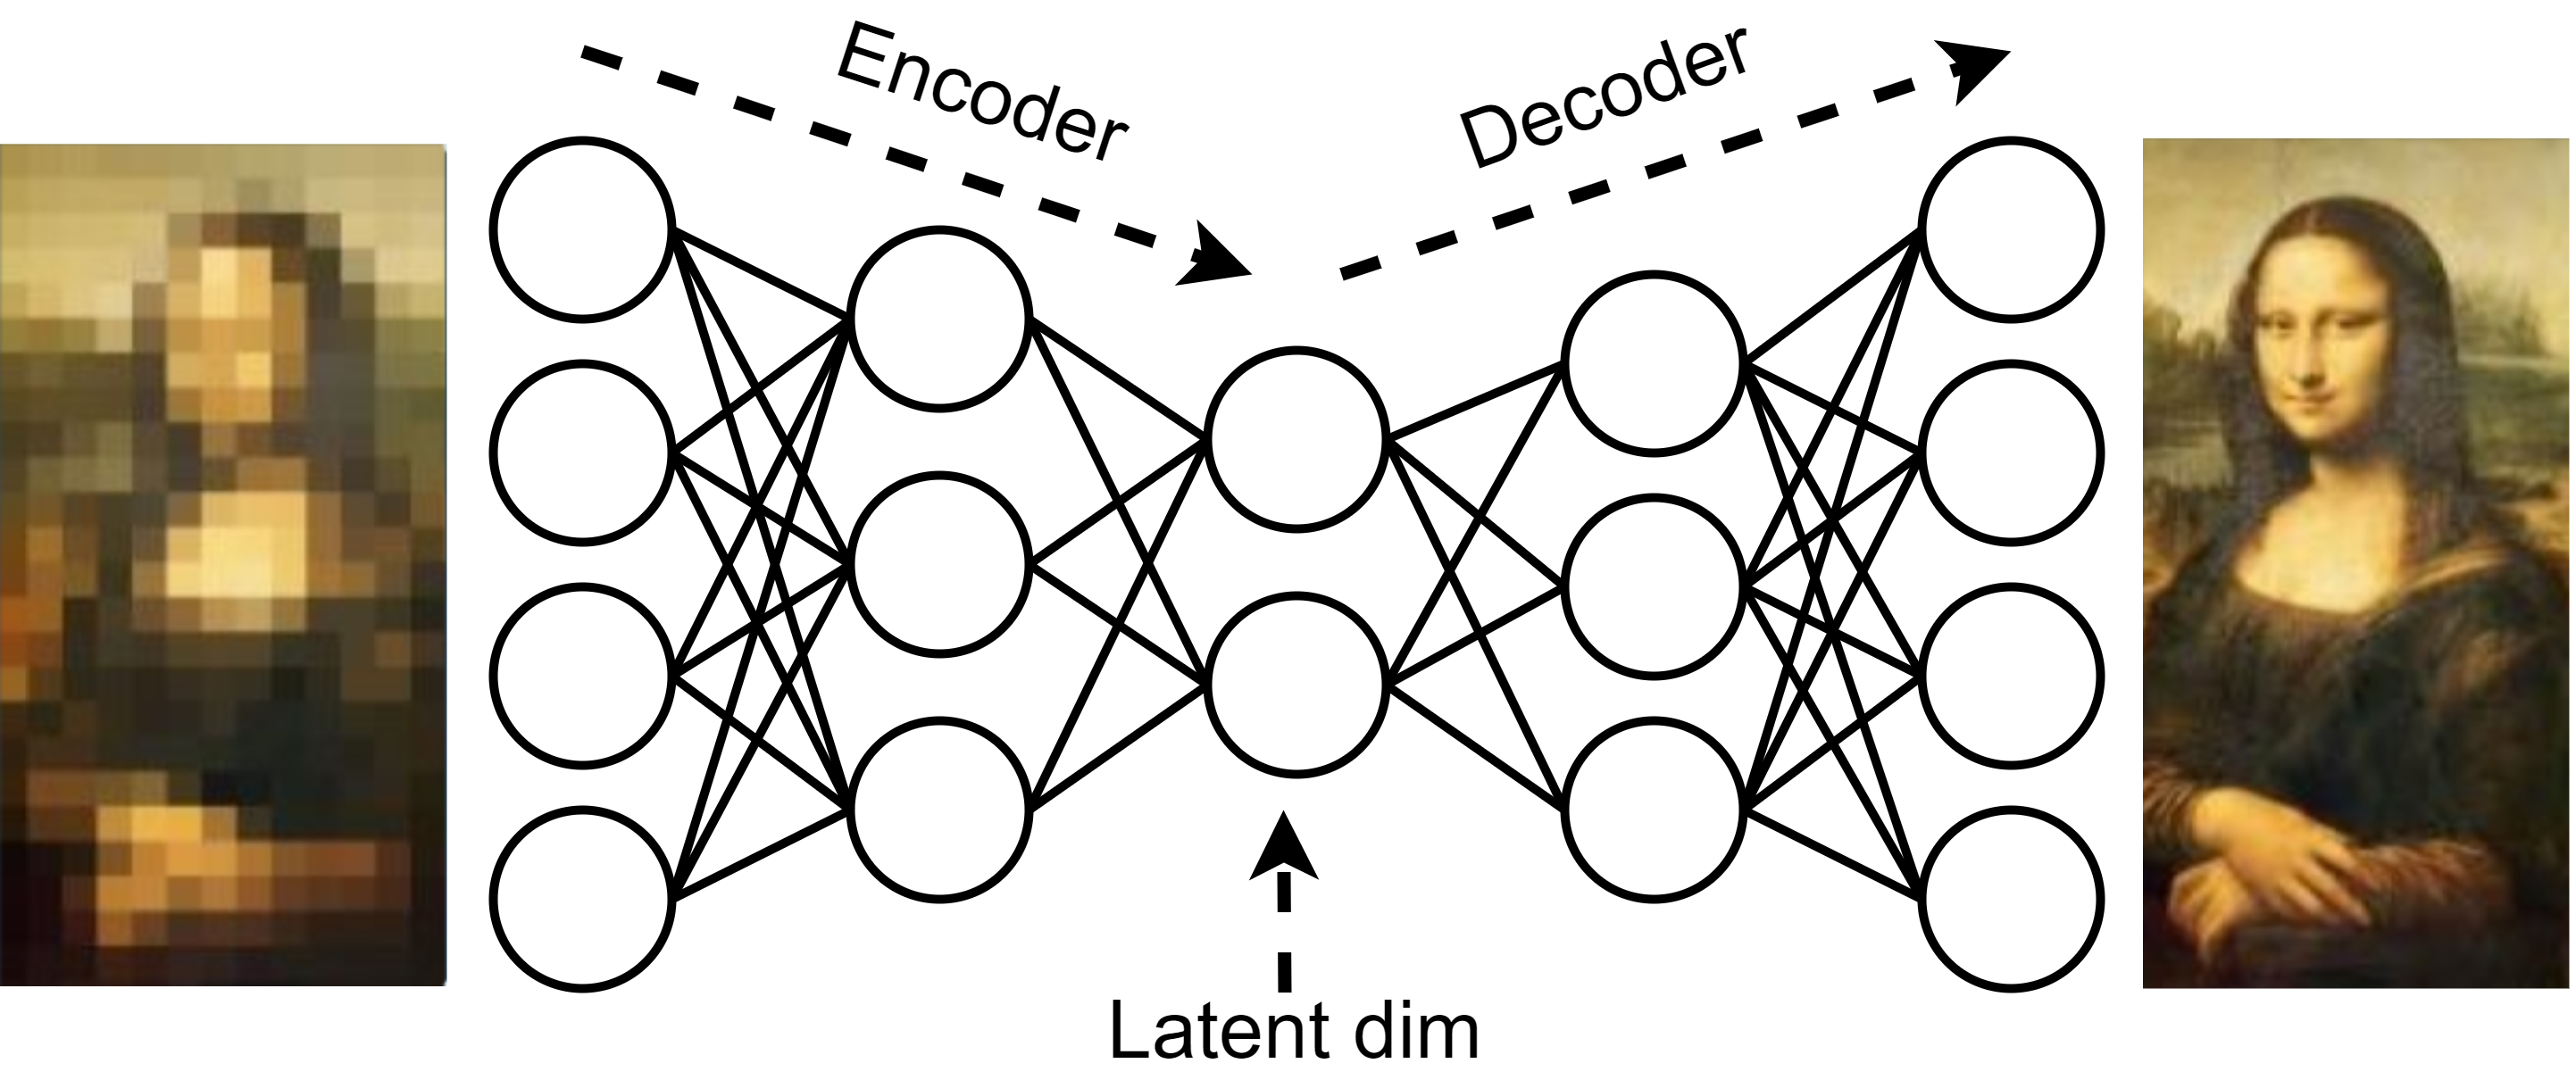
\includegraphics[width=0.8\textwidth]{Slides/figures/GAN/Autoencoder.png}
        \caption{Modelo de Autoencoder capaz de reconstruir una imagen de baja resolución.}
    \end{figure}

\end{frame}

\begin{frame}{Variational Autoencoder}
    
    \begin{itemize}
        \item Aprende a generalizar gracias al uso de una \alert{función de densidad}.
        
        \item Genera datos \alert{indistinguibles} de los de entrada.
        
        \item Genera nuevos datos \alert{sin copiar} directamente los ejemplos.
    \end{itemize}
    
    \begin{figure}
        \centering
        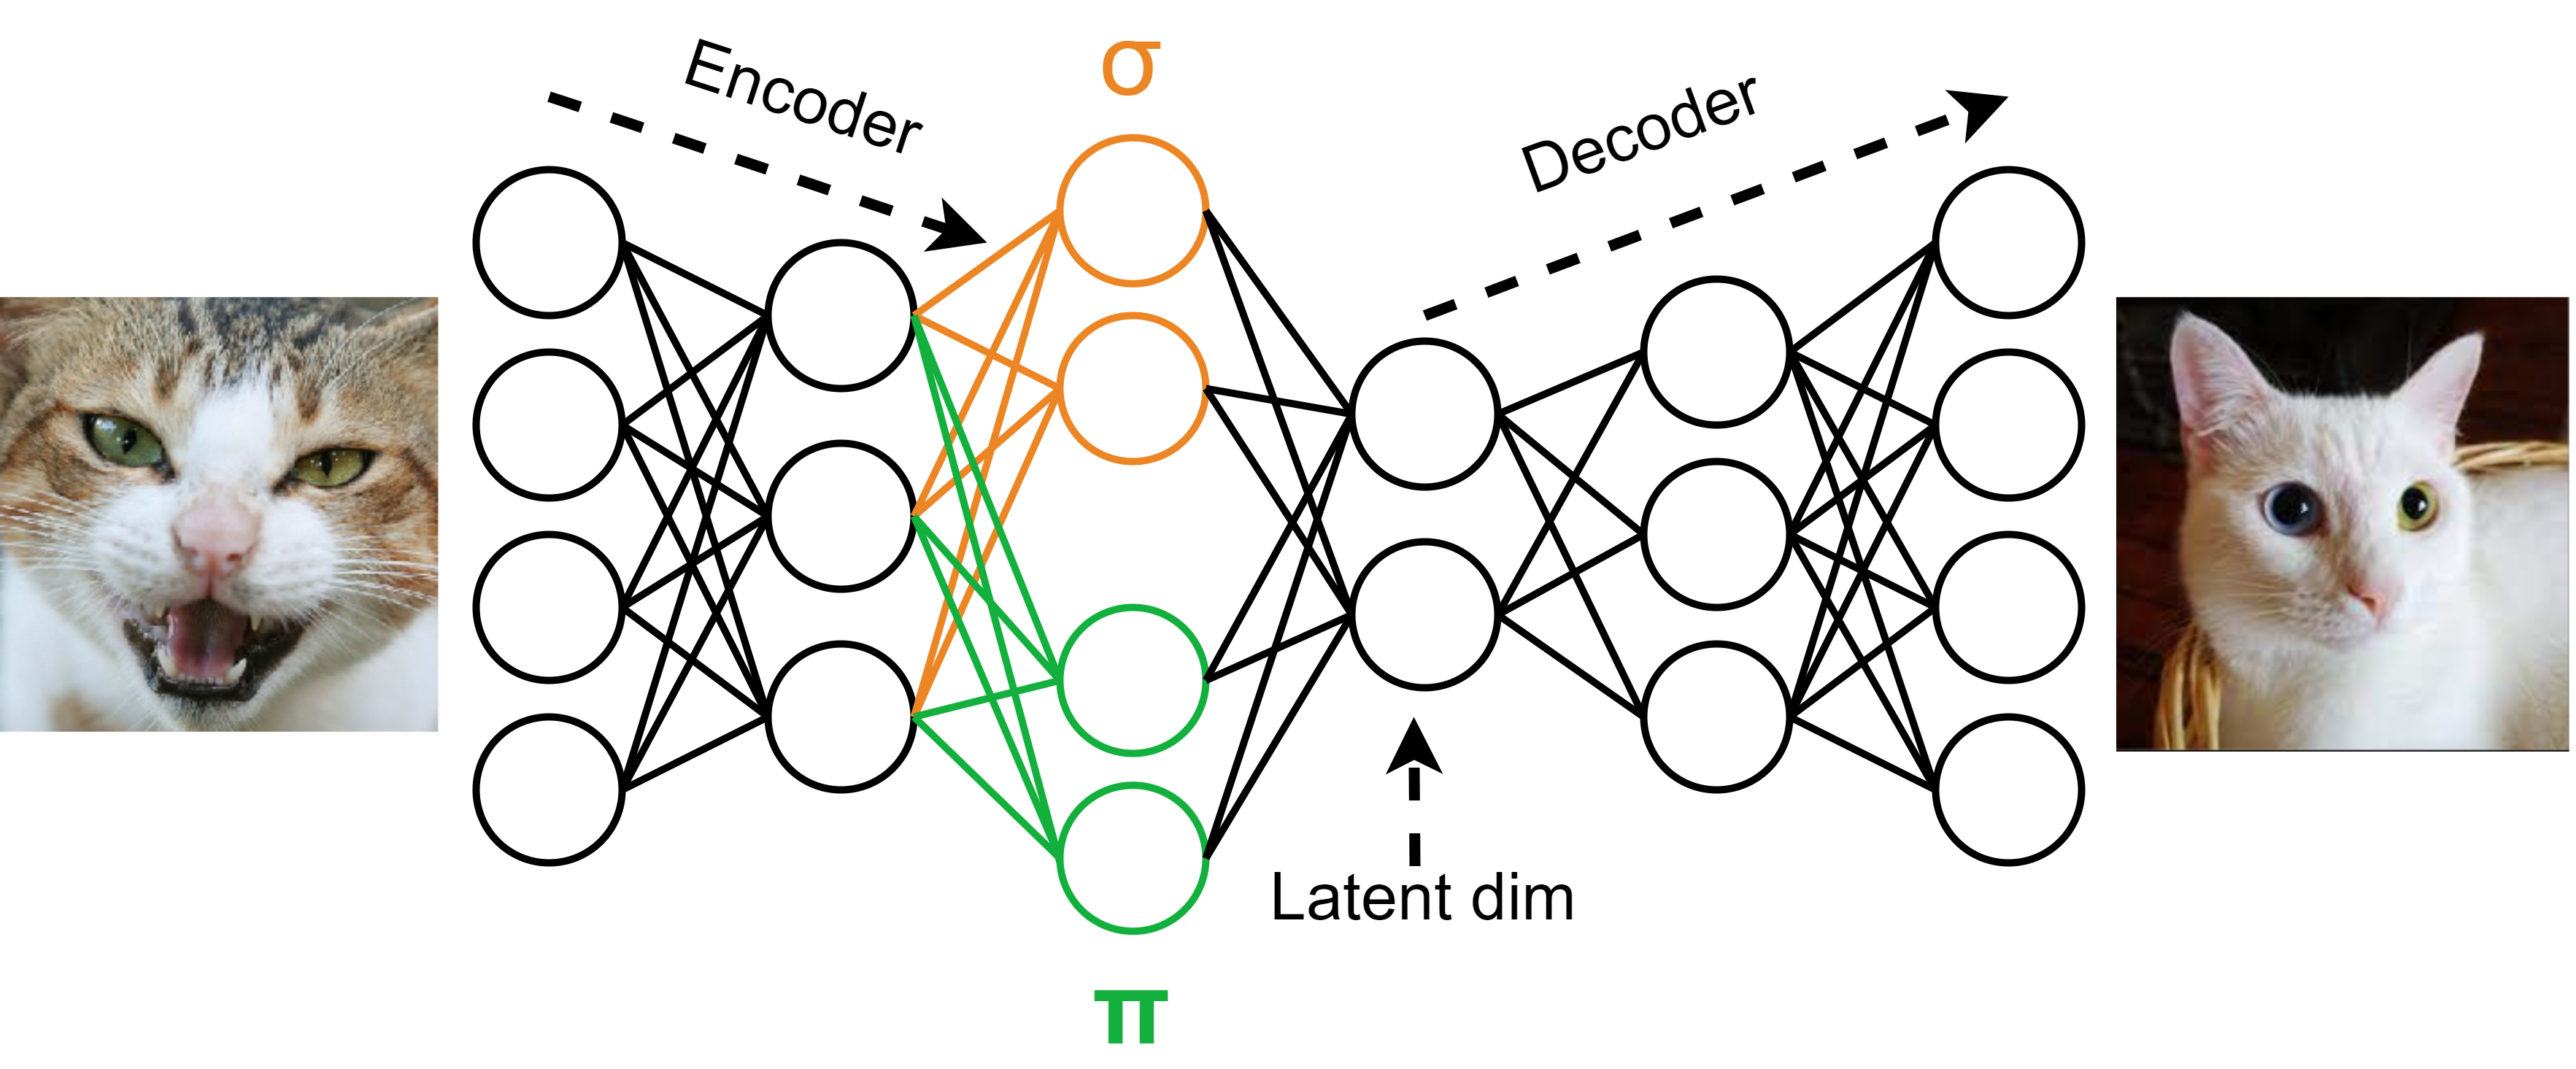
\includegraphics[width=\textwidth]{Slides/figures/GAN/Variational Autoencoder.png}
        \caption{Modelo de Variational Autoencoder capaz de generar imágenes de gatos.}
    \end{figure}
    \hfill

\end{frame}

\begin{frame}{Modelos generativos: principales problemas}
    
    \begin{itemize}
        \item Estos modelos no tienen la \alert{calidad suficiente}.
        \item Se buscan alternativas capaces de generar resultados \alert{más nítidos}.
        \item La aproximación de \alert{aprender} directamente la distribución genera resultados \alert{poco diversos}.
    \end{itemize}

\end{frame}

\section{\gls{gan}: Fundamentos}

\begin{frame}{Definición}

    \begin{itemize}
        \item Las redes \gls{gan} fueron propuestas en el año 2014 por Ian Goodfellow\cite{goodfellow2014generative}.
        \item Se definen como un modelo \alert{neuronal generativo} basado en la \alert{teoría de juegos} que tiene como objetivo \alert{replicar} una distribución de datos.
        \item Se basa en un juego de \alert{suma cero} que involucra \alert{2 redes neuronales distintas}.
    \end{itemize}
    
\end{frame}

\begin{frame}{Redes \gls{gan}: Intuición previa}

    \vfill
    {\Large Ejemplo: Falsificador vs. policía}
    
    \begin{itemize}
        \item Se quieren hacer \alert{falsificaciones} de billetes.
        \item Se busca que la policía sea \alert{incapaz de distinguir} entre los billetes falsos y los reales.
    \end{itemize}
    
    \begin{figure}
        \centering
        
\includegraphics[width=\textwidth]{Slides/figures/GAN/PoliciaLadronBilletes 1.PNG}
    \end{figure}
    
\end{frame}

\begin{frame}{Redes \gls{gan}: Intuición previa}

    {\Large Falsificador}
    \hfill
    
    \begin{columns}[T]
    \begin{column}{.3\textwidth}
    
    \begin{figure}
        \centering
        
\includegraphics[width=\textwidth]{Slides/figures/GAN/Falsificador.PNG}
    \end{figure}
    
    \end{column}
    \hfill
    \begin{column}{.68\textwidth}
    
    \begin{itemize}
        \item Excelente artista.
        \item Es capaz de \alert{generar nuevos} billetes.
        \item Inicialmente \alert{no sabe} lo que es un billete.
    \end{itemize}

    \end{column}
    \end{columns}
    
    \vfill
    \centering
    \textbf{\Large Quiere \alert{engañar} al policía con billetes \alert{falsos}.}
    
\end{frame}

\begin{frame}{Redes \gls{gan}: Intuición previa}

    {\Large Policía}
    \hfill
    
    \begin{columns}[T]
    \begin{column}{.3\textwidth}
    
    \begin{figure}
        \centering
        
\includegraphics[width=\textwidth]{Slides/figures/GAN/Policia.PNG}
    \end{figure}
    
    \end{column}
    \hfill
    \begin{column}{.68\textwidth}
    
    \begin{itemize}
        \item \alert{Discrimina} la veracidad de cada billete.
        \item Inicialmente \alert{no sabe} lo que es un billete.
    \end{itemize}

    \end{column}
    \end{columns}
    
    \vfill
    \centering
    \textbf{\Large Quiere \alert{separar} los billetes \alert{falsos} de los \alert{verdaderos}.}
    
\end{frame}

\begin{frame}{Redes \gls{gan}: Intuición previa}
    
    \begin{itemize}
        \item El ladrón intenta \alert{engañar} al policía generando billetes que se \alert{parezcan} a los reales.
        \item Si engaña al policía sabe que ese billete es de \alert{buena calidad}.
    \end{itemize}
    
    \begin{figure}
        \centering
        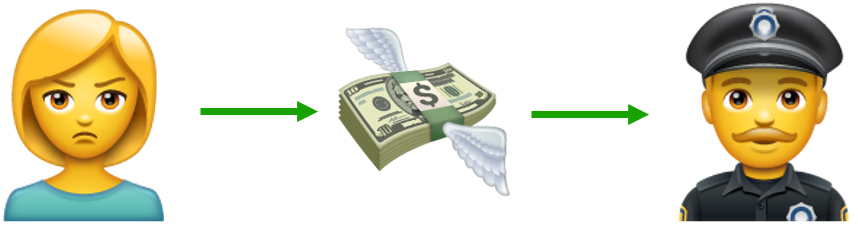
\includegraphics[width=\textwidth]{Slides/figures/GAN/PoliciaLadronBilletes 2.PNG}
    \end{figure}
    
\end{frame}

\begin{frame}{Redes \gls{gan}: Intuición previa}
    
    \begin{itemize}
        \item El policía intenta no ser engañado \alert{discriminando} las diferencias \alert{más sutiles} entre los billetes.
        \item Si es \alert{engañado} aprende cuáles son esos \alert{detalles} que hacen que el billete sea falso.
    \end{itemize}
    
    \begin{figure}
        \centering
        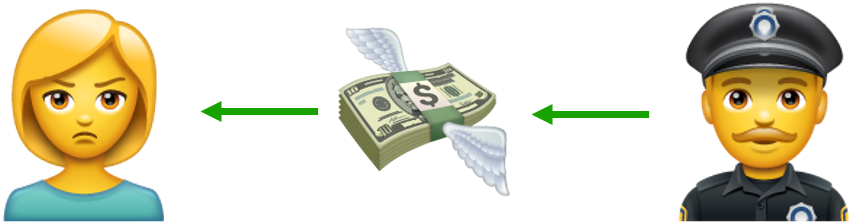
\includegraphics[width=\textwidth]{Slides/figures/GAN/PoliciaLadronBilletes 3.PNG}
    \end{figure}
    
\end{frame}

\begin{frame}{Redes \gls{gan}: Intuición previa}
    
    \begin{itemize}
        \item El policía y el falsificador \alert{compiten} por quien consigue vencer al otro.
        \item A medida que el tiempo pasa los billetes del falsificador son \alert{más realistas} pero el policía aprende a \alert{diferenciar mejor} los pequeños detalles.
        \item La competición entre ambos hacen que mejoren de manera \alert{simultánea y paralela}.
    \end{itemize}
    
    \begin{figure}
        \centering
        
\includegraphics[width=\textwidth]{Slides/figures/GAN/PoliciaLadronBilletes 1.PNG}
    \end{figure}
    
\end{frame}

\begin{frame}{Esquema general de una red \gls{gan}}
    
    \begin{figure}
        \centering
        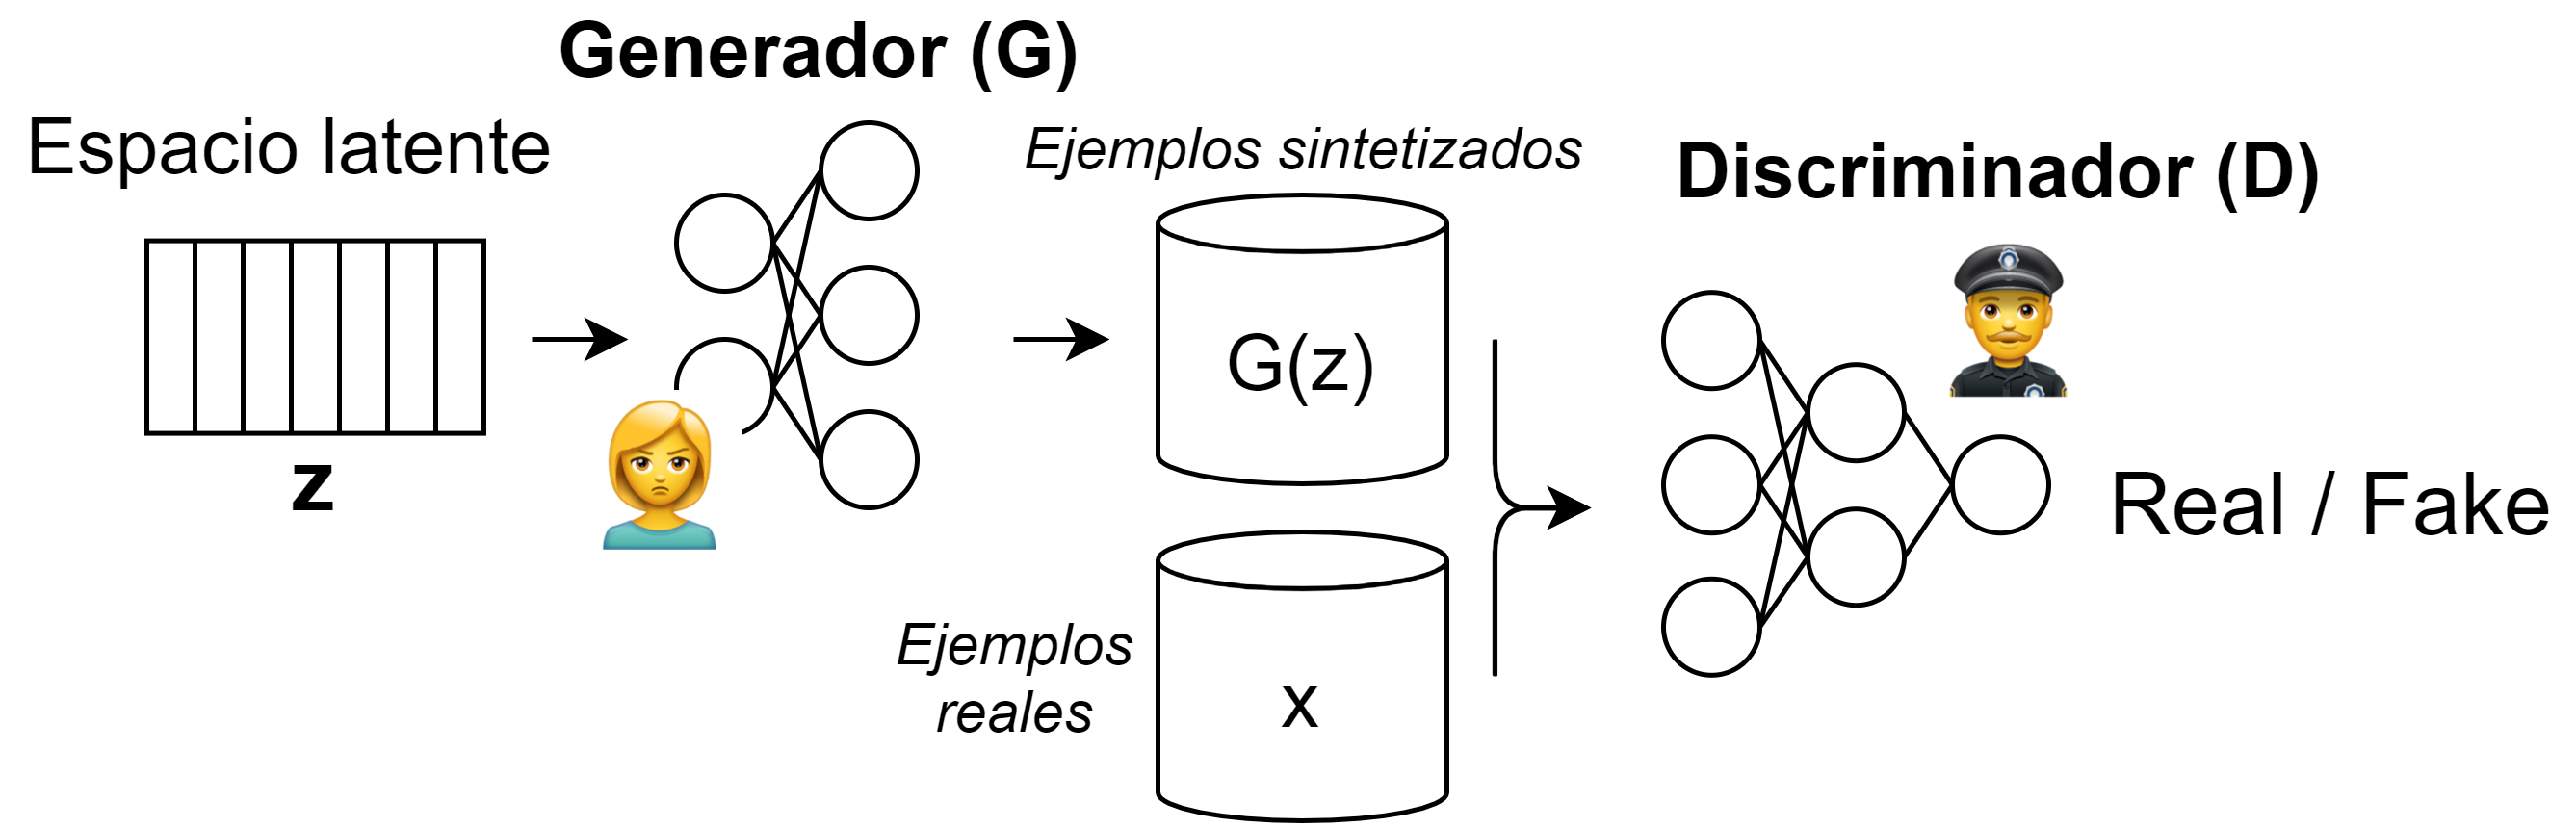
\includegraphics[width=\textwidth]{Slides/figures/GAN/GAN architecture 1.png}
        \caption{Arquitectura GAN.}
    \end{figure}
    
\end{frame}

\begin{frame}{Generador}
    
    \begin{figure}
        \centering
        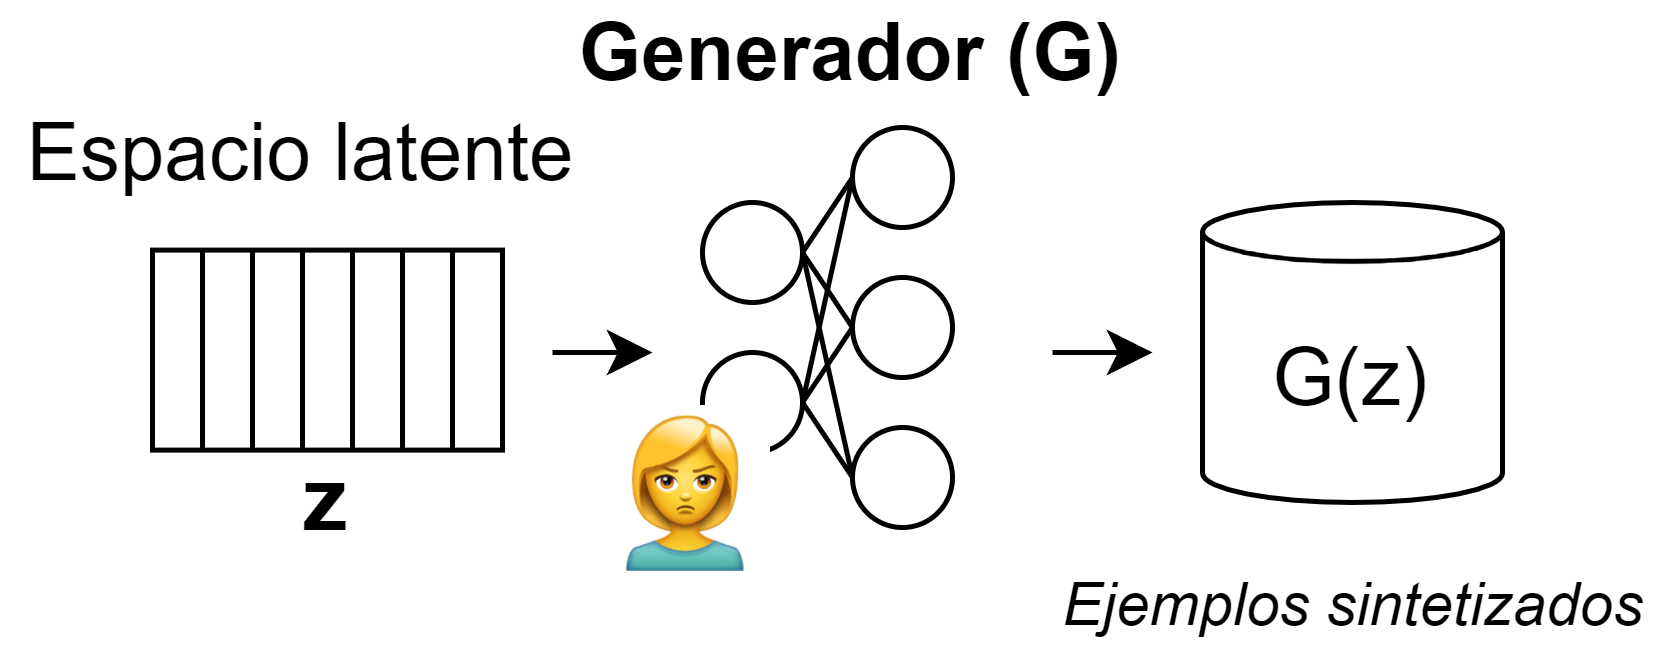
\includegraphics[width=\textwidth]{Slides/figures/GAN/Generador.png}
        \caption{Arquitectura del generador.}
    \end{figure}
    
    \alert{Genera} datos a partir de un \alert{espacio latente} que le proporciona aleatoriedad.
    
\end{frame}

\begin{frame}{Discriminador}
    
    \begin{figure}
        \centering
        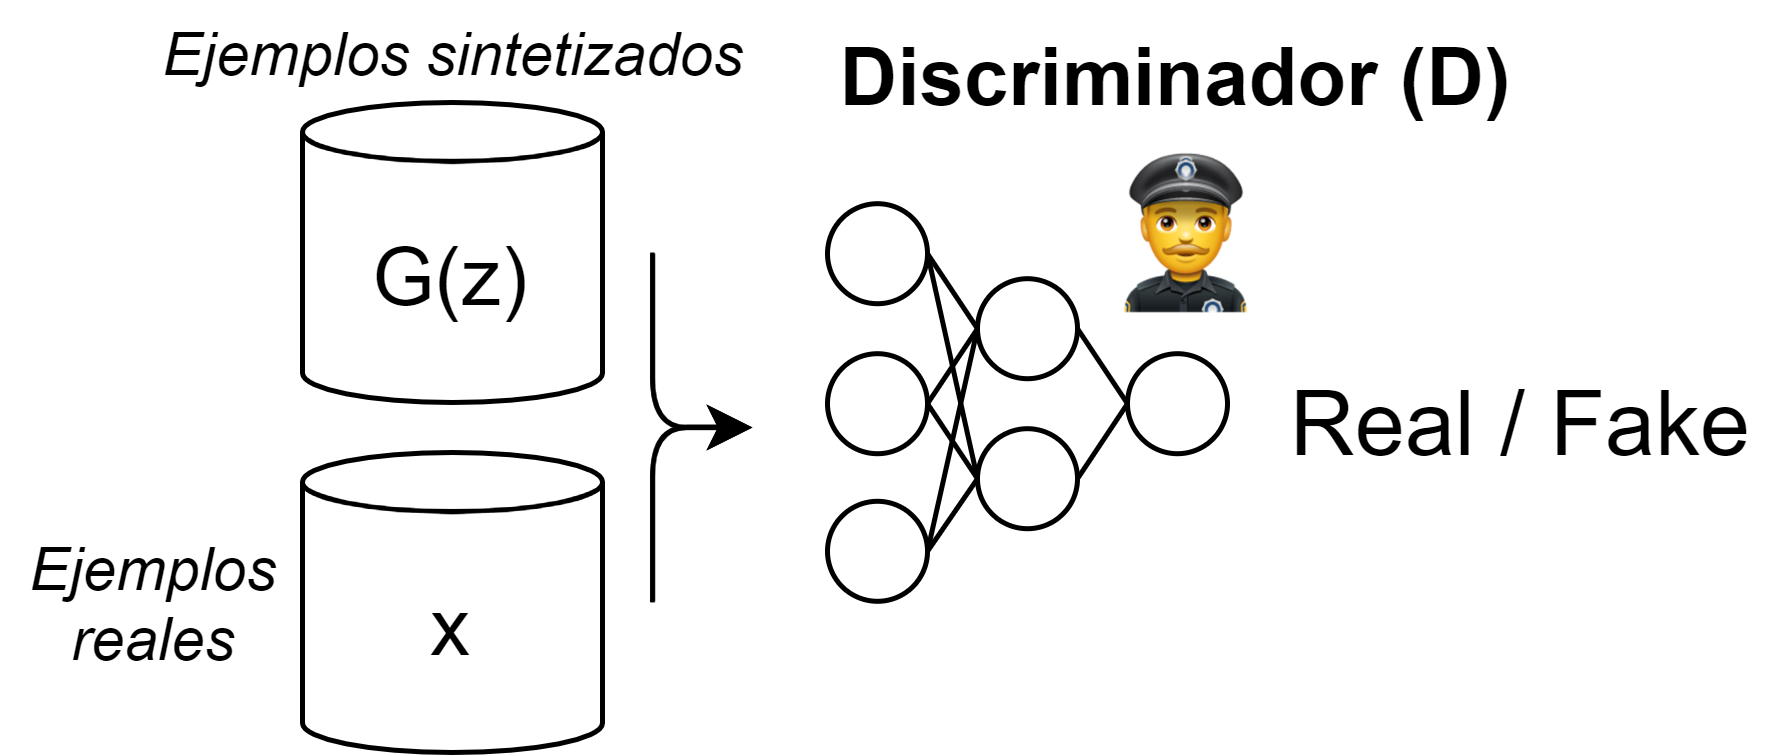
\includegraphics[width=\textwidth]{Slides/figures/GAN/Discriminador.png}
        \caption{Arquitectura del discriminador.}
    \end{figure}
    
    \alert{Discrimina} los datos a partir de la \alert{distribución real} y la \alert{distribución generada por el generador}.
    
\end{frame}

\begin{frame}{Esquema general de una red \gls{gan}}
    
    \begin{figure}
        \centering
        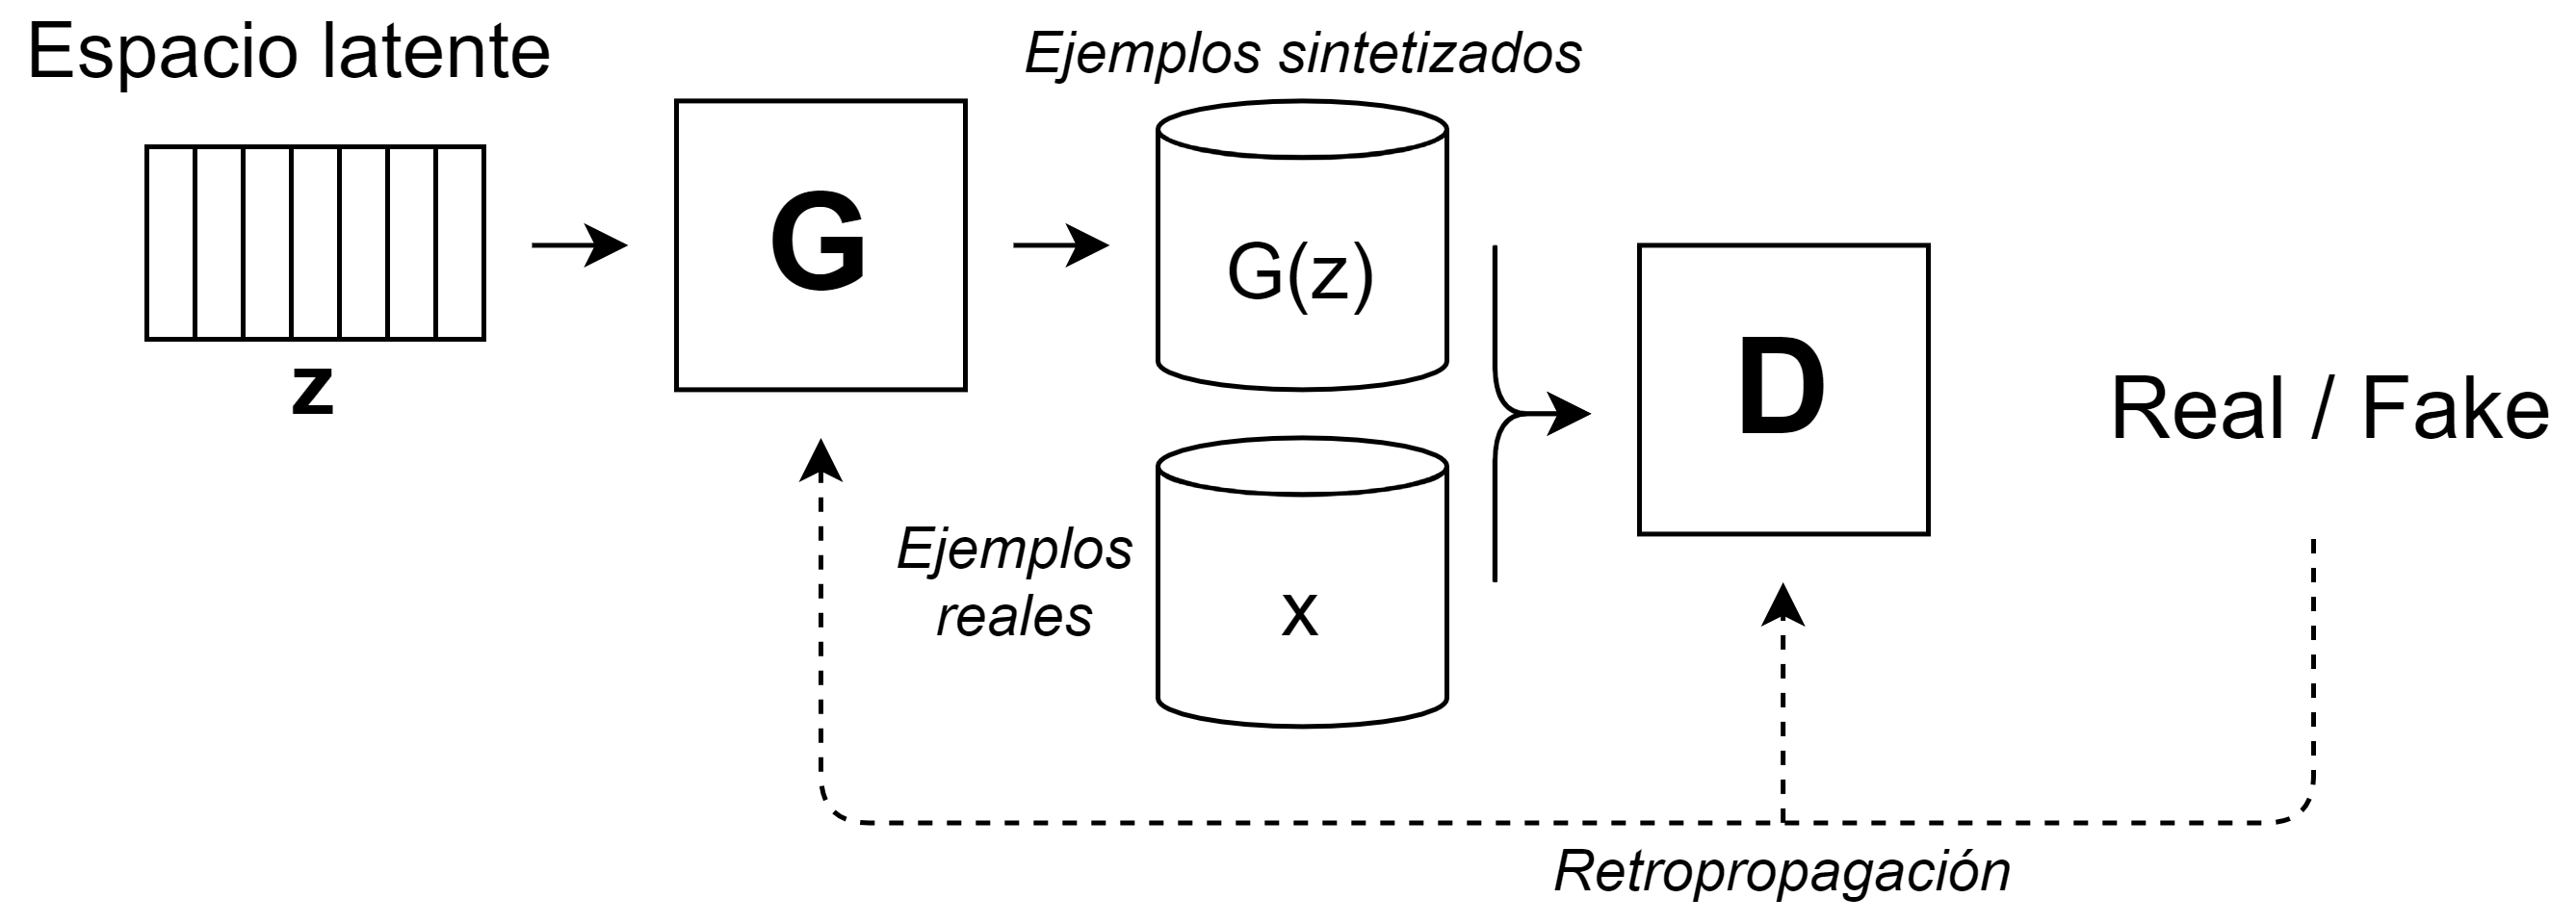
\includegraphics[width=\textwidth]{Slides/figures/GAN/GAN architecture 2.png}
        \caption{Arquitectura GAN.}
    \end{figure}
    
    \begin{itemize}
        \item Durante el entrenamiento de una \gls{gan} se produce una \alert{competición} entre \alert{G} y \alert{D}.
        \item En ella ambos modelos mejoran \alert{progresivamente} de manera \alert{simultánea}.
    \end{itemize}
    
\end{frame}

\section{\gls{gan}: Entrenamiento}

\begin{frame}{Entrenamiento del Discriminador}
    
    \begin{figure}
        \centering
        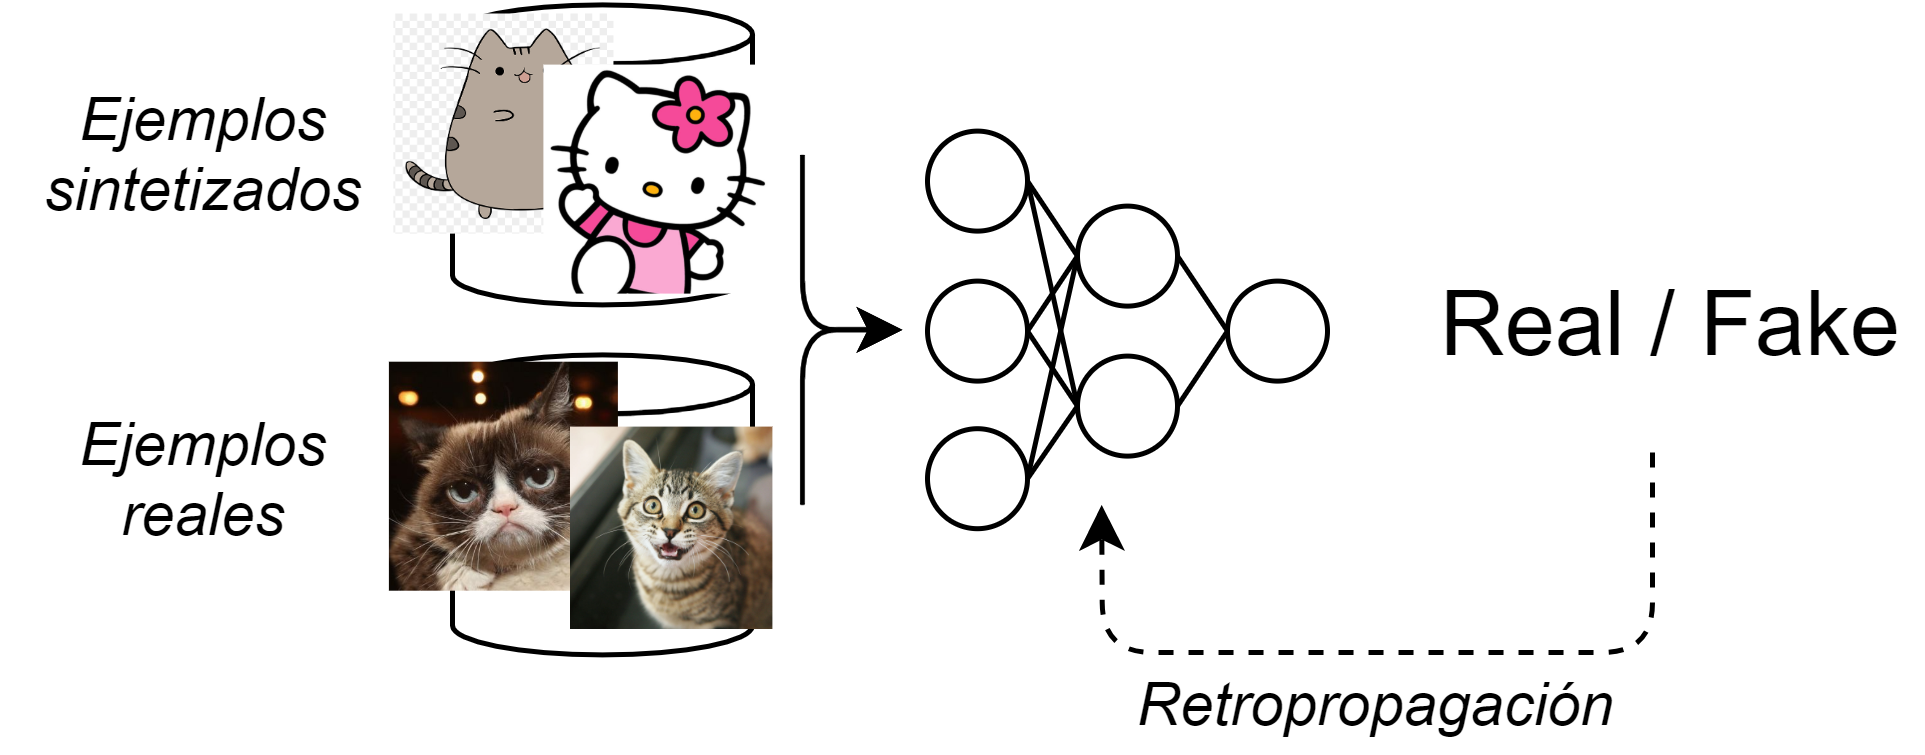
\includegraphics[width=0.8\textwidth]{Slides/figures/GAN/Discriminador Iteracion.png}
        \caption{Entrenamiento de D.}
    \end{figure}
    
    \begin{itemize}
        \item El D no es más que un \alert{clasificador} binario.
        \item Su objetivo es \alert{diferenciar} qué datos son \alert{reales} y cuales \alert{falsos}.
        \item Durante su entrenamiento realiza un aprendizaje para diferenciar ambas \alert{distribuciones}.
        \item Se tiene que adaptar \alert{constantemente} a las mejoras en las imágenes generadas por el G.
    \end{itemize}
    
\end{frame}

\begin{frame}{Entrenamiento del Discriminador}
    \begin{columns}[T]
    \begin{column}{.55\textwidth}
    
    \begin{figure}
        \centering
        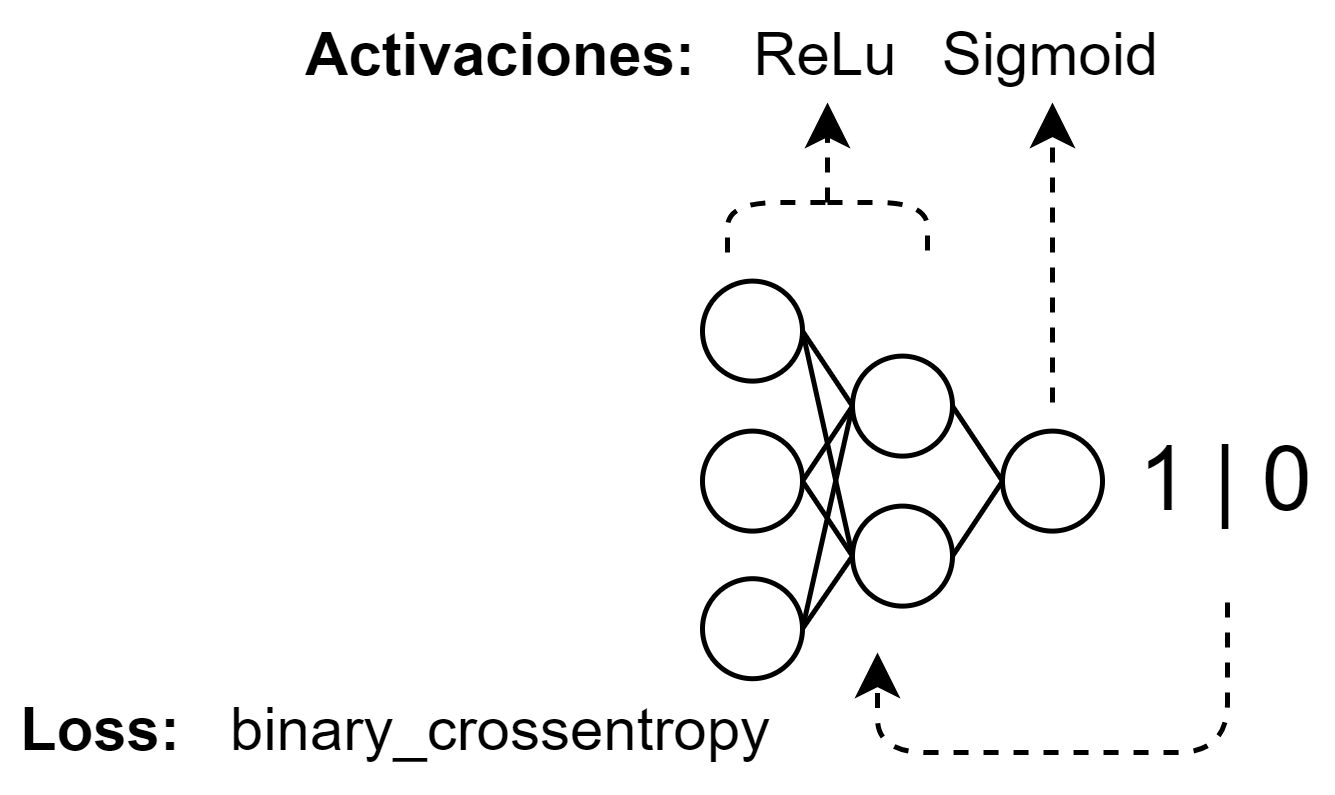
\includegraphics[width=\textwidth]{Slides/figures/GAN/Discriminador Red.png}
        \caption{Pérdida y activaciones de D.}
    \end{figure}
    
    \end{column}
    \hfill
    \begin{column}{.45\textwidth}
    
    \begin{figure}
        \centering
        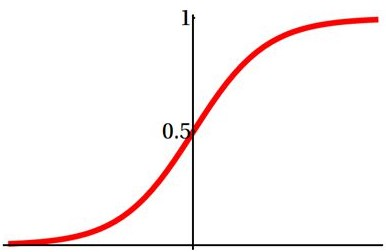
\includegraphics[width=\textwidth]{Slides/figures/GAN/Sigmoid.jpg}
        \caption{Función de activación sigmoide.}
    \end{figure}
    
    \end{column}
    \end{columns}
    
    \begin{itemize}
        \item Las activaciones de las capas ocultas y de entrada son \alert{cualquiera} que permita actualizar los pesos \alert{correctamente}.
        
        \item Al ser una clasificación \alert{binaria} la activación de la capa de salida será la sigmoide (en el rango [0, 1]).
        
        \item La función de \alert{pérdida} es la Entropía cruzada binaria.
    \end{itemize}
    
\end{frame}

\begin{frame}{Entrenamiento del Generador}
    
    \begin{figure}
        \centering
        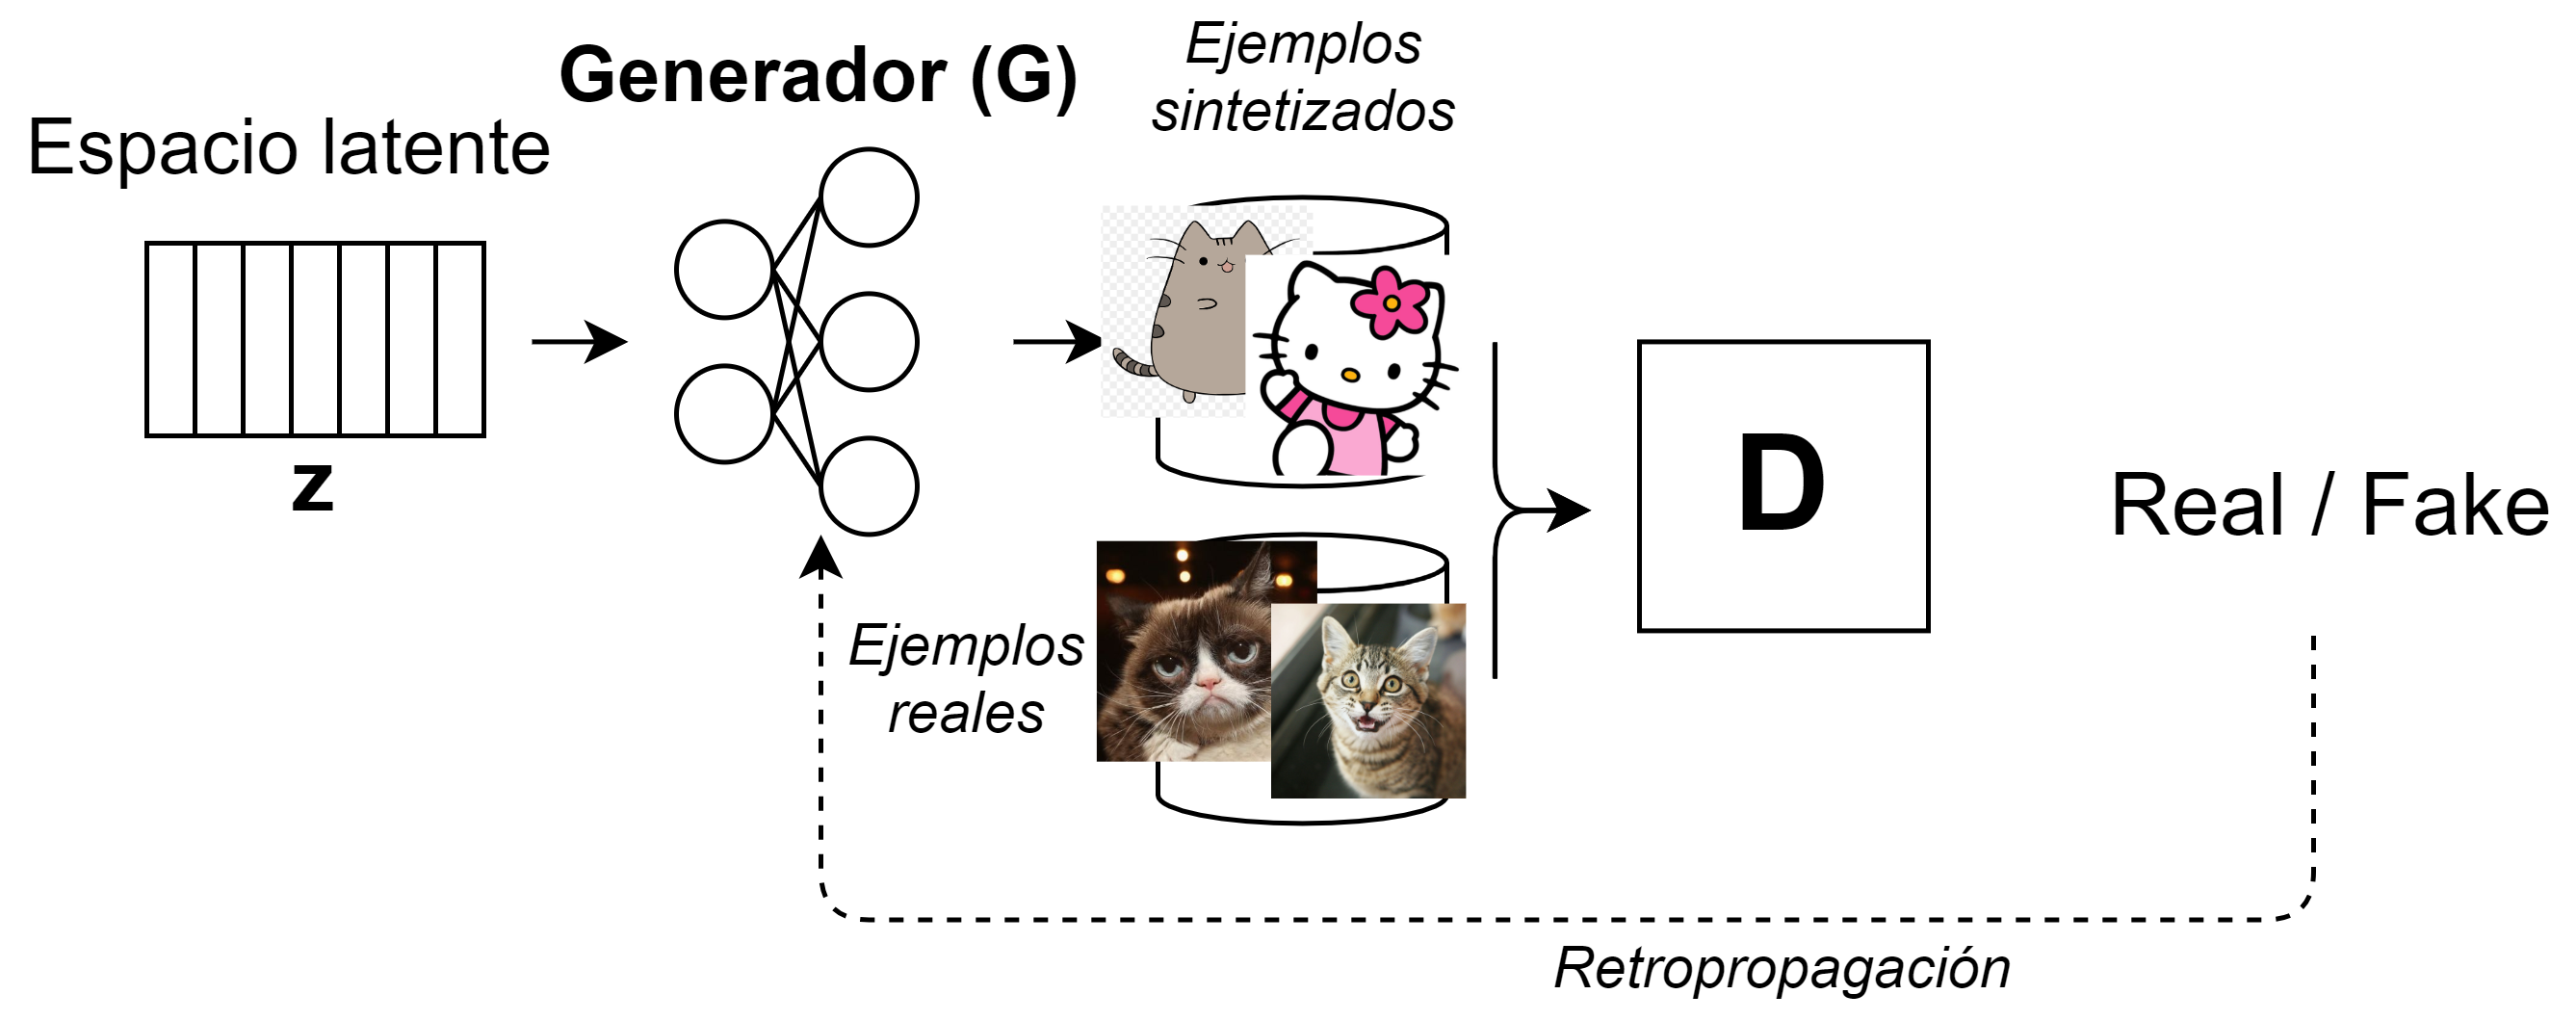
\includegraphics[width=0.9\textwidth]{Slides/figures/GAN/Generador Iteracion.png}
        \caption{Entrenamiento de G.}
    \end{figure}
    
    \begin{itemize}
        \item El G genera \alert{nuevos} datos a partir del espacio latente.
        \item La \alert{actualización} de pesos se hace a través del \alert{D}.
        \item Su entrenamiento \alert{depende} de si el \alert{D} es capaz de diferenciar los datos.
    \end{itemize}
    
\end{frame}

\begin{frame}{Entrenamiento del Generador}
    
    {\Large \alert{Espacio latente}}
    
    Se genera a través de ruido Gausiano o uniforme.
    
    \begin{columns}[T]
    \begin{column}{.48\textwidth}
    
    \begin{figure}
        \centering
        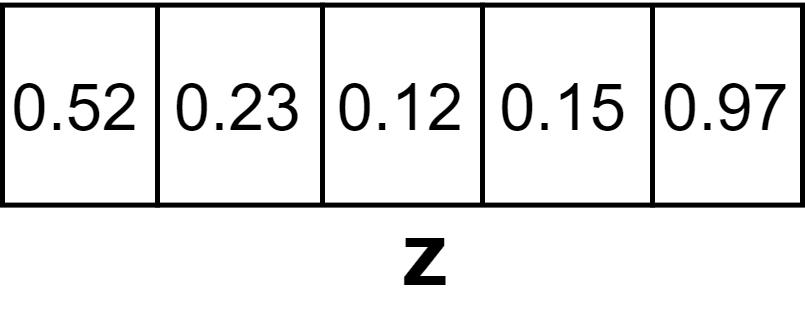
\includegraphics[width=\textwidth]{Slides/figures/GAN/Latent Space.png}
        \caption{Vector de espacio latente.}
    \end{figure}
    
    \end{column}
    \hfill
    \begin{column}{.48\textwidth}
    
    \begin{itemize}
        \item Es un \alert{vector n-dimensional} de números reales.
        \item Actúa de \alert{semilla} para la generación de nuevos datos.
        \item Introduce la aleatoriedad necesaria a la red.
    \end{itemize}
    
    \end{column}
    \end{columns}
    
\end{frame}

\begin{frame}{Entrenamiento del Generador}
    \begin{columns}[T]
    \begin{column}{.55\textwidth}
    
    \begin{figure}
        \centering
        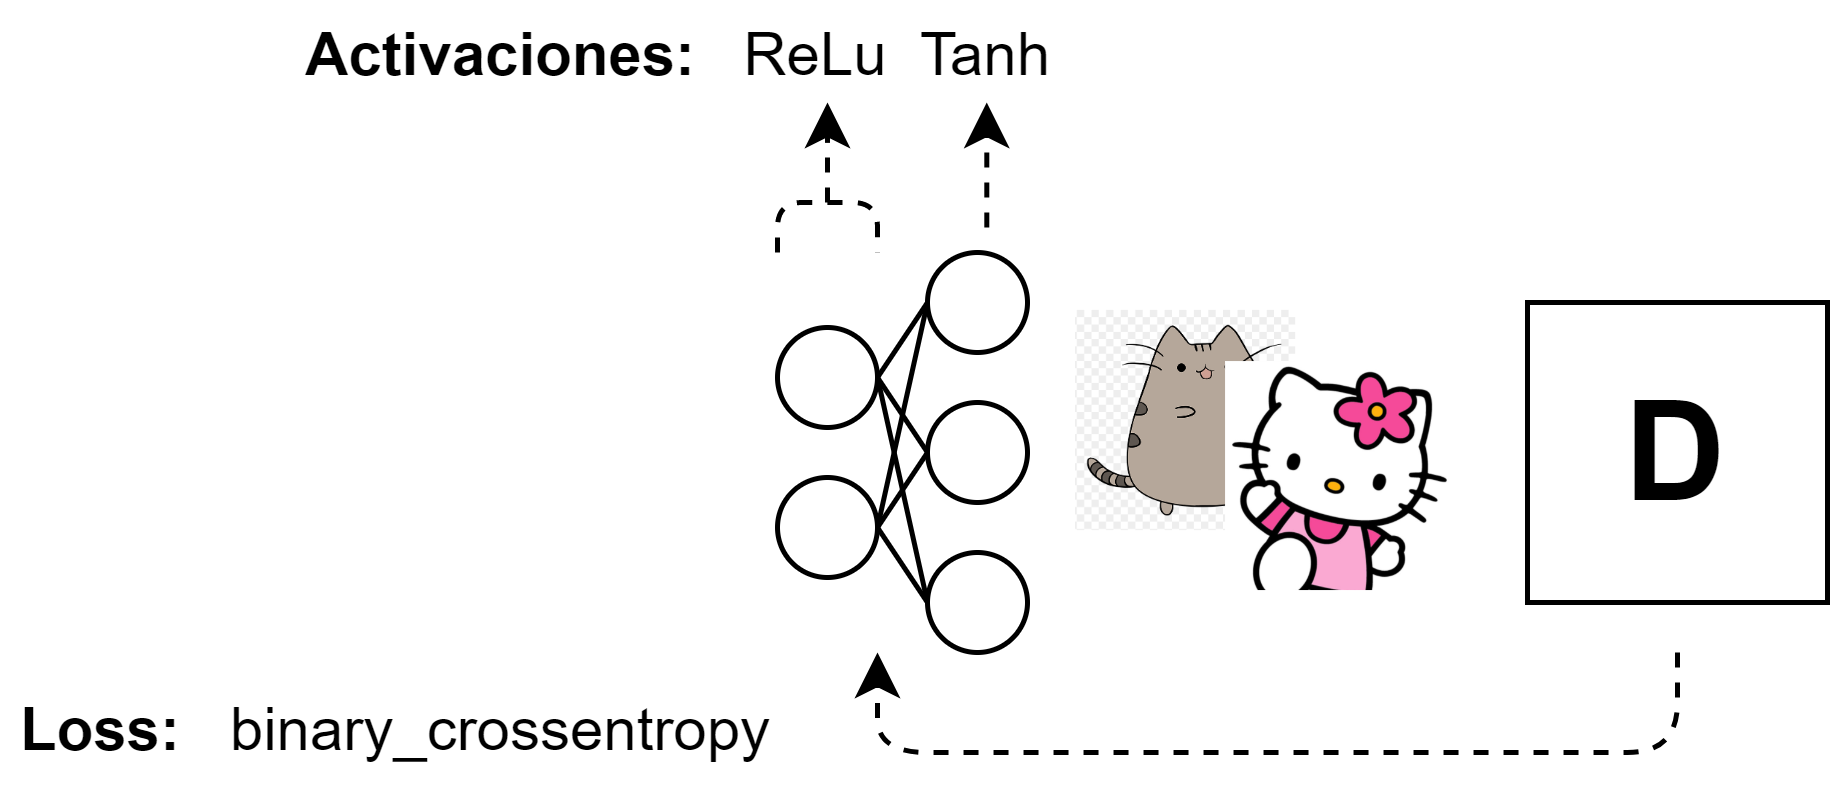
\includegraphics[width=\textwidth]{Slides/figures/GAN/Generador Red.png}
        \caption{Pérdida y activaciones de G.}
    \end{figure}
    
    \end{column}
    \hfill
    \begin{column}{.45\textwidth}
    
    \begin{figure}
        \centering
        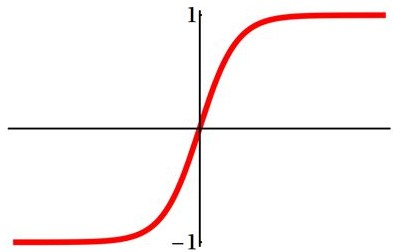
\includegraphics[width=\textwidth]{Slides/figures/GAN/Tanh.jpg}
        \caption{Función de activación tangencial.}
    \end{figure}
    
    \end{column}
    \end{columns}
    
    \begin{itemize}
        \item Las activaciones de las capas ocultas y de entrada son \alert{cualquiera} que permita actualizar los pesos \alert{correctamente}.
        
        \item La \alert{activación} de la capa de salida será aquella que \alert{permita generar} los datos de manera \alert{correcta}.
        
        \item La función de \alert{pérdida} es la Entropía cruzada binaria, con origen en la salida del D.
    \end{itemize}
    
\end{frame}

\begin{frame}{Entrenamiento: Primeras iteraciones}

    \begin{columns}[T]
    \begin{column}{.48\textwidth}
    
    \begin{figure}
        \centering
        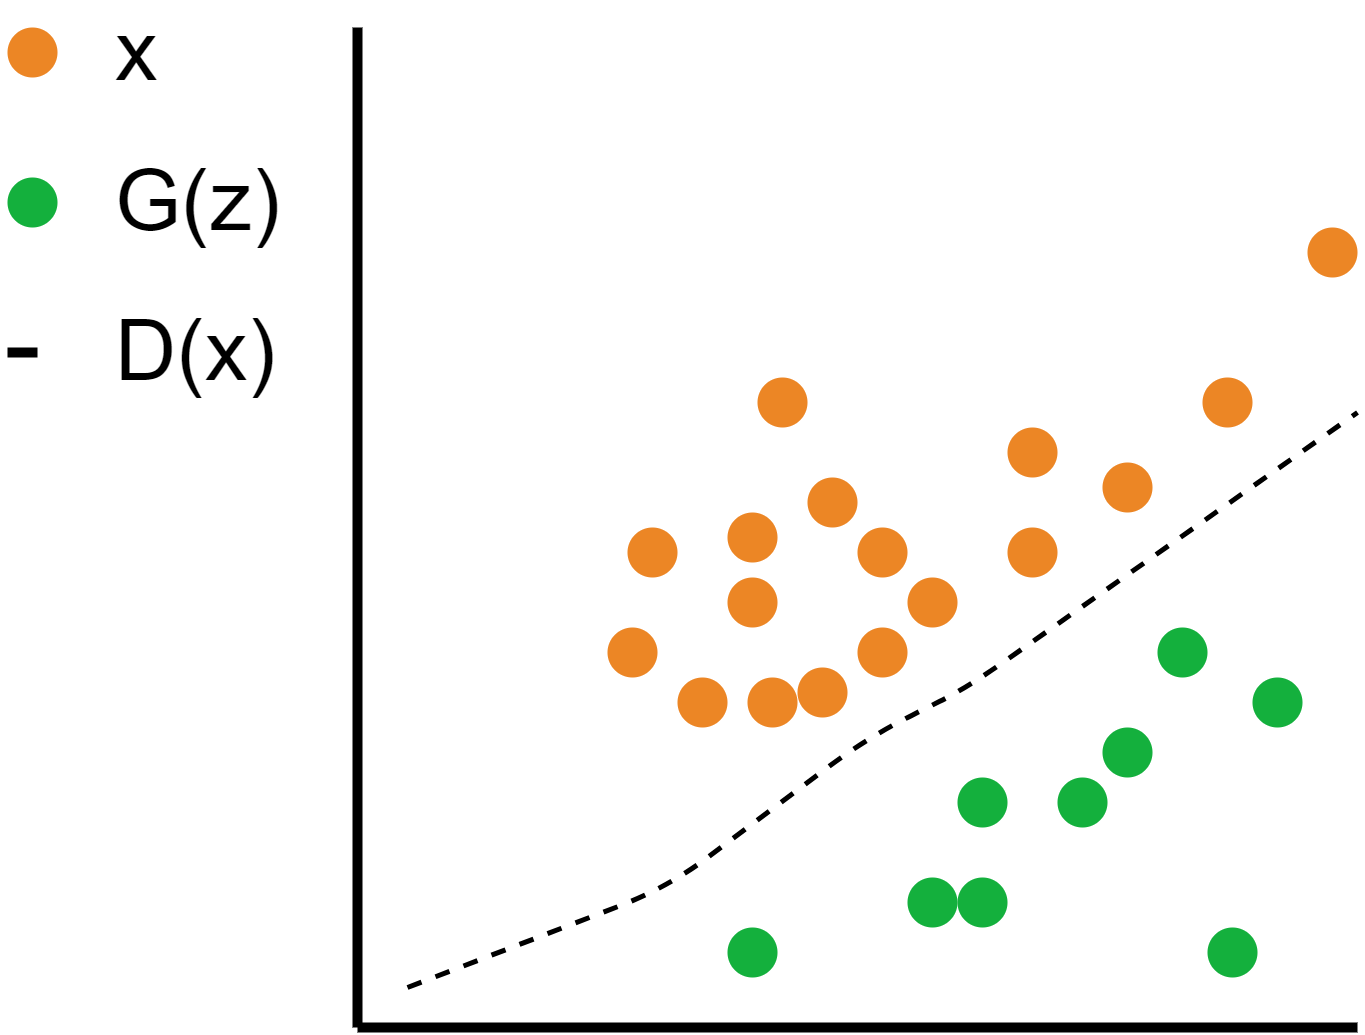
\includegraphics[width=\textwidth]{Slides/figures/GAN/Entreno distribucion 1.png}
        \caption{Distribución de datos reales (naranja) y generados (verde) durante las primeras iteraciones de un entrenamiento.}
    \end{figure}
    
    \end{column}
    \hfill
    \begin{column}{.48\textwidth}
    
    \begin{itemize}
        \item Es muy fácil la \alert{diferenciación} entre ambas distribuciones.
        \item Los datos generados son de \alert{muy mala calidad} (ruido).
    \end{itemize}

    \end{column}
    \end{columns}
    
\end{frame}

\begin{frame}{Entrenamiento: Iteraciones intermedias}

    \begin{columns}[T]
    \begin{column}{.48\textwidth}
    
    \begin{figure}
        \centering
        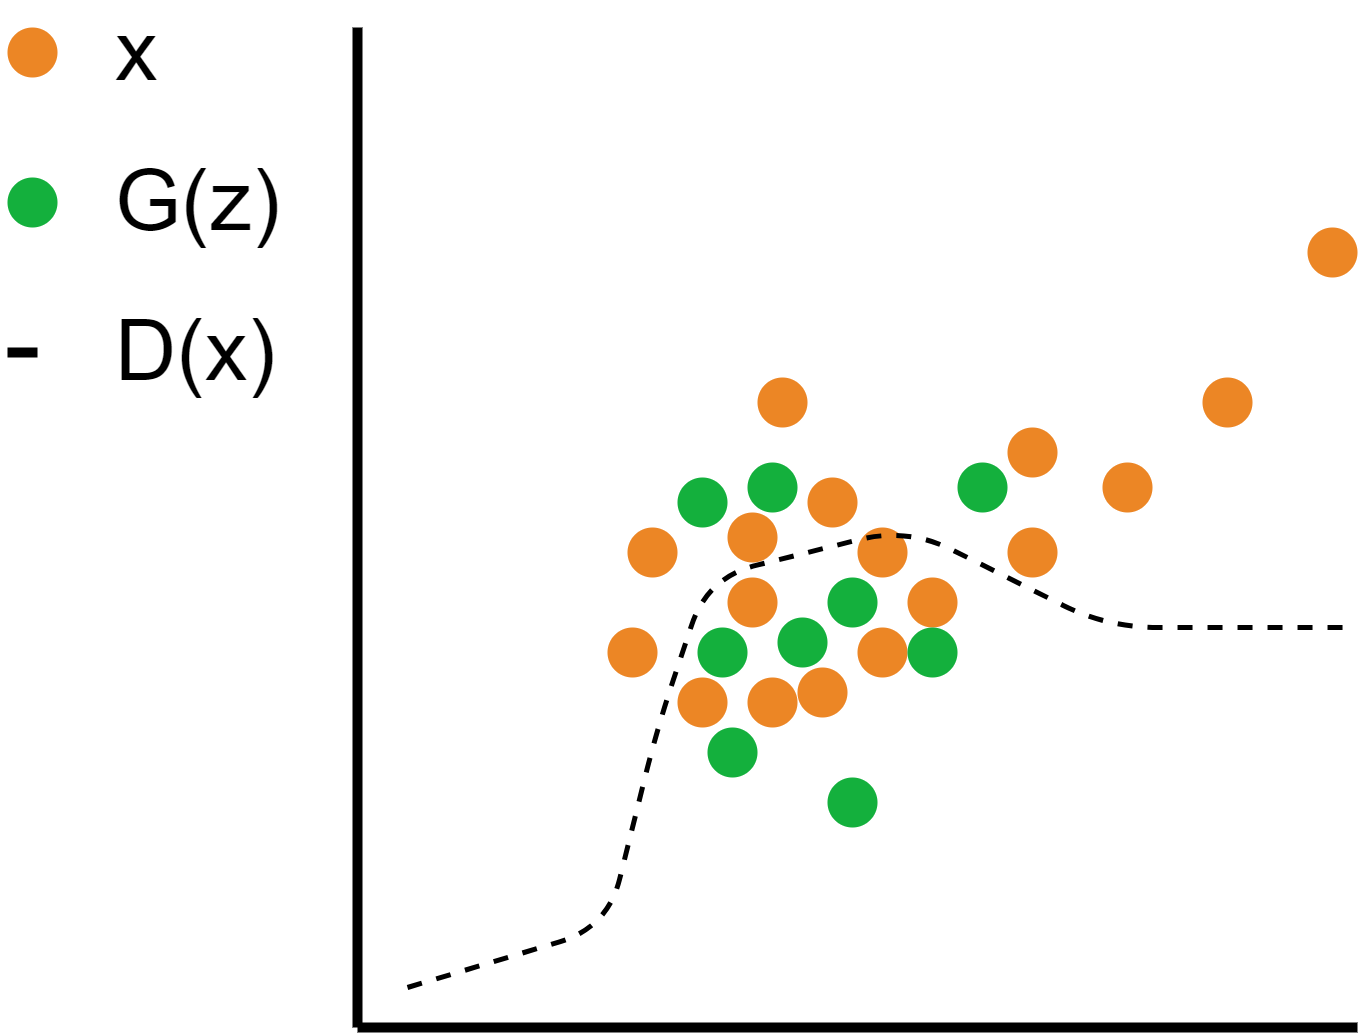
\includegraphics[width=\textwidth]{Slides/figures/GAN/Entreno distribucion 2.png}
        \caption{Distribución de datos reales (naranja) y generados (verde) durante las iteraciones intermedias de un entrenamiento.}
    \end{figure}
    
    \end{column}
    \hfill
    \begin{column}{.48\textwidth}
    
    \begin{itemize}
        \item El generador comienza a generar datos que \alert{engañan} al discriminador.
        \item Todavía existen \alert{diferencias notables} entre ambas distribuciones.
    \end{itemize}

    \end{column}
    \end{columns}
    
\end{frame}

\begin{frame}{Entrenamiento: Final del entrenamiento}

    \begin{columns}[T]
    \begin{column}{.48\textwidth}
    
    \begin{figure}
        \centering
        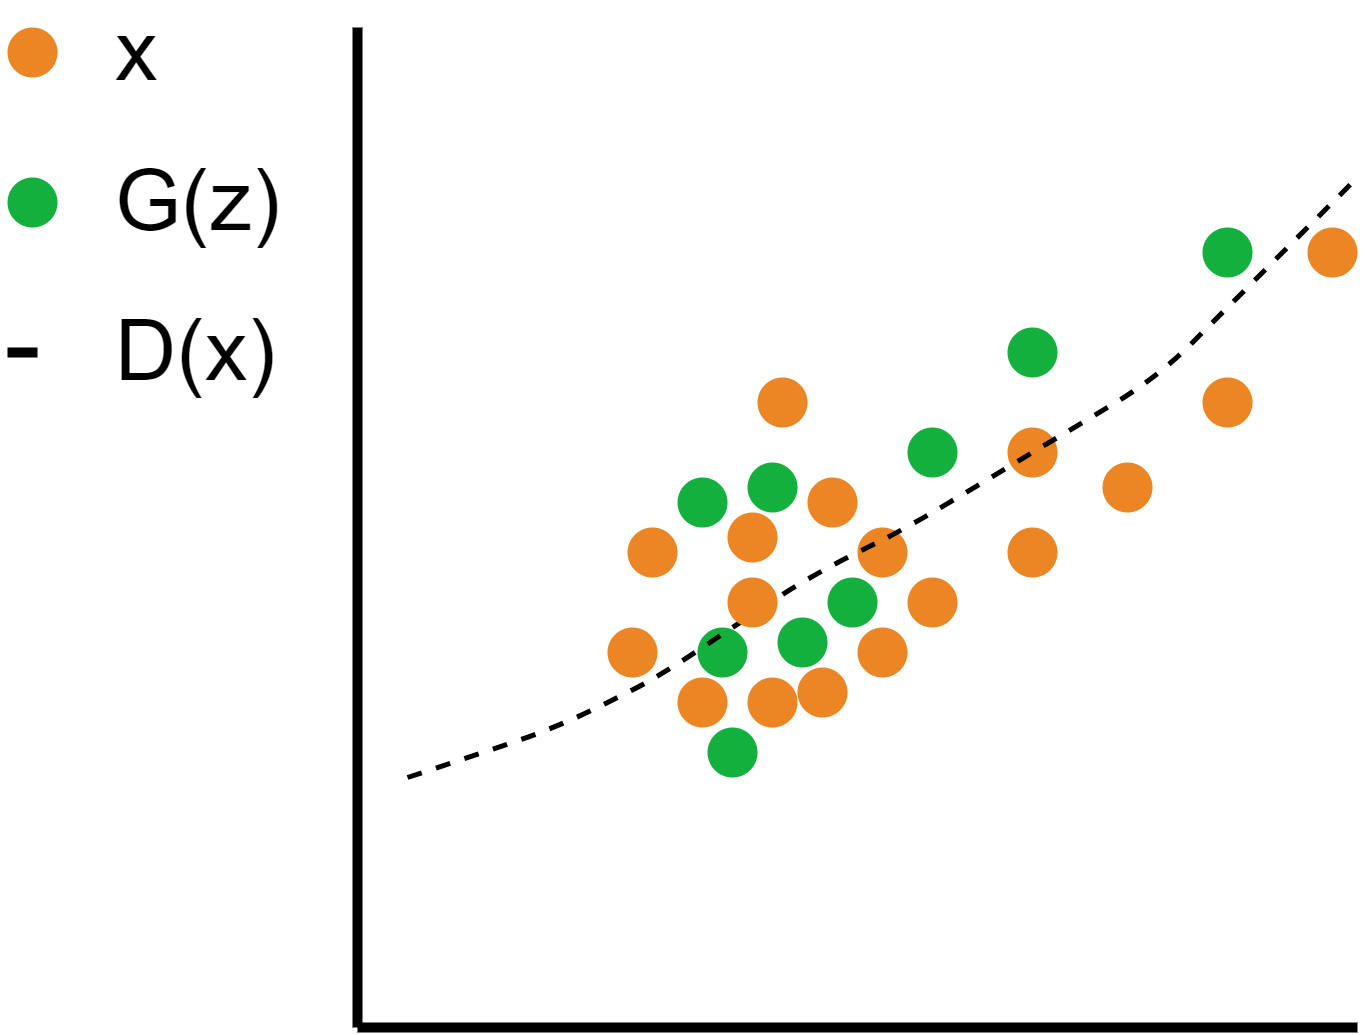
\includegraphics[width=\textwidth]{Slides/figures/GAN/Entreno distribucion 3.png}
        \caption{Distribución de datos reales (naranja) y generados (verde) tras haber finalizado un entrenamiento exitoso.}
    \end{figure}
    
    \end{column}
    \hfill
    \begin{column}{.48\textwidth}
    
    \begin{itemize}
        \item Ambas distribuciones son \alert{indistinguibles}.
        \item El discriminador es \alert{incapaz} de \alert{diferenciar} de qué distribución proceden los datos.
        \item Se ha llegado al \alert{equilibrio de Nash}\cite{cournot1897researches}.
    \end{itemize}

    \end{column}
    \end{columns}
    
\end{frame}

\begin{frame}{Fundamentación matemática}
    
    \hfill
    \vfill
    {\Large Minimax game}
    \begin{itemize}
        \item El generador busca \alert{minimizar} la siguiente expresión:
    \end{itemize}
    
    \begin{equation}
        \Large \log [1-D(G(z))]
    \end{equation}
    
    \begin{itemize}
        \item El discriminador busca \alert{maximizar} la siguiente expresión:
    \end{itemize}
    
    \begin{equation}
        \Large \log [D(x)]+\log [1-D(G(z))]
    \end{equation}
    
\end{frame}

\begin{frame}{Fundamentación matemática}
    
    \hfill
    \vfill
    {\Large Minimax game}
    \begin{itemize}
        \item El juego de \alert{minimax} entre ambos modelos se denota por la siguiente expresión:
    \end{itemize}
    
    \begin{equation}
        \Large \min _{G} \max _{D} L(D, G)=\log [D(x)]+\log [1-D(G(x))]
    \end{equation}
    
    \begin{itemize}
        \item \alert{G} intenta \alert{engañar} a \alert{D}.
        \item \alert{D} intenta \alert{discriminar} correctamente ambas \alert{distribuciones}.
    \end{itemize}
    
\end{frame}

\begin{exercise}
\href{https://colab.research.google.com/drive/1WF-FahMjwXlpPWHWGg9qESUQhKFxGqJW}{GANs con Densas}
\end{exercise}

\begin{exercise}
\href{https://colab.research.google.com/drive/1FxURNzD_FenraqJF9lHa81Dx4jNUjop-}{Deep Convolutional GANs - DCGAN}
\end{exercise}

\section{\gls{gan}: Problemas principales}

\begin{frame}{Problemas de las GAN}

    Las \gls{gan} cuentan con una serie de \alert{problemas comunes}. Estos suelen presentarse en los entrenamientos de una \gls{gan} debido a las particularidades de su \alert{arquitectura}.
    
    Se revisarán los siguientes:
    \begin{itemize}
        \item Inestabilidad
        \item Problemas derivados del gradiente:
        \begin{itemize}
            \item Gradient explosion
            \item Gradient vanishing
        \end{itemize}
        \item Mode Collapse
    \end{itemize}
    
\end{frame}

\begin{frame}{Inestabilidad}

    {\Large El problema de la \alert{inestabilidad} se debe a que las \gls{gan} cuentan con \alert{2} redes neuronales al mismo tiempo.}
    
    \begin{itemize}
        \item Las redes neuronales de por sí son modelos \alert{inestables}.
        \item Al hacer que dos modelos \alert{interactúen} entre sí se \alert{aumenta esta inestabilidad}.
        \item Mantener una \alert{coordinación} entre ambas redes es un \alert{proceso delicado}.
    \end{itemize}
    
\end{frame}

\begin{frame}{Inestabilidad}
    
    Para intentar evitar la \alert{inestabilidad} se suelen tomar una serie de \alert{precauciones} que intenten \alert{equilibrar el entrenamiento}:
    
    \begin{itemize}
        \item Que las \alert{arquitecturas} de la D y la G tengan la \alert{misma forma} pero inversa.
        \item En caso de que el D sea muy \alert{certero} (caso más habitual), limitar su potencia haciendo uso de \alert{regularización}.
    \end{itemize}
    
    Que las dos redes no estén en \alert{sincronía} puede hacer que ninguna entrene correctamente, ya que el G \alert{necesita} que el D falle de vez en cuando y viceversa.
    
\end{frame}

\begin{frame}{Problemas del gradiente}

    Los problemas \alert{derivados del gradiente} son comunes a todas las redes neuronales. Estos están \alert{directamente influenciados} por el número de capas de la red.
    
    Se diferencian dos tipos:
    \begin{itemize}
        \item Gradient explosion.
        \item Gradient vanishing.
    \end{itemize}
    
    Al realizarse la \alert{retropropagación} los \alert{valores de pérdida} pasan de unas capas a otras. En este algoritmo las derivadas de cada neurona pueden llegar a \alert{descontrolarse}.
    
    \begin{equation}
        W_{x}^{\prime}=W_{x}-\mathrm{\alpha}\left(\frac{\partial \text {Loss}}{\partial W_{x}}\right)
    \end{equation}
    
\end{frame}

\begin{frame}{Problemas del gradiente: Gradient explosion}

    \begin{figure}
        \centering
        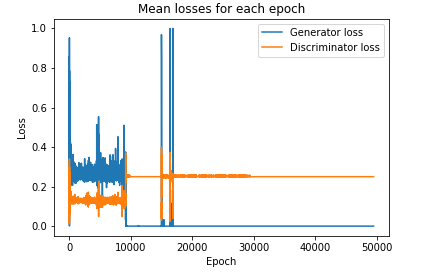
\includegraphics[width=0.6\textwidth]{Slides/figures/GAN/GradientExplosion.png}
        \caption{Gradient explosion.}
    \end{figure}
    
    El \alert{gradient explosion}, también conocido como \alert{exploding gradients} sucede cuando la actualización de pesos toma valores \alert{muy elevados}.
    
    Se identifica con valores de pérdidas de \alert{NaN o muy exageradas}.
    
\end{frame}

\begin{frame}{Problemas del gradiente: Gradient Vanishing}

    \begin{figure}
        \centering
        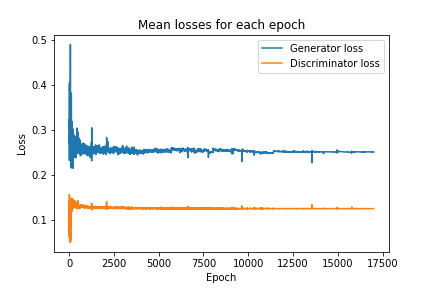
\includegraphics[width=0.6\textwidth]{Slides/figures/GAN/GradientVanishing.png}
        \caption{Gradient vanishing.}
    \end{figure}
    
    Cuando sucede \alert{gradient vanishing}, también llamado \alert{vanishing gradients}, la actualización de pesos se hace \alert{nula} por tener valores \alert{muy pequeños}.
    
    Se identifica cuando la pérdida es \alert{constante en el tiempo}.
    
\end{frame}

\begin{frame}{Mode Collapse}

    \begin{figure}
        \centering
        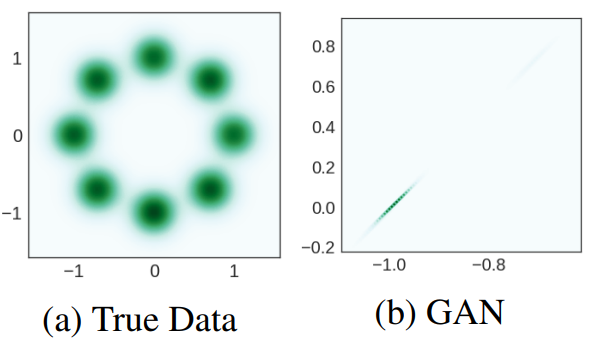
\includegraphics[width=0.6\textwidth]{Slides/figures/GAN/Mode Collapse.png}
        \caption{Mode collapse, figura extraída de \cite{srivastava2017veegan}.}
    \end{figure}

    El \alert{colapso modal} sucede cuando la información generada sólo pertenece a un \alert{subgrupo} de la total.
    
\end{frame}

\section{\gls{gan}: Aplicaciones}

\begin{frame}{\gls{gan} en el mundo real}

    Las \alert{\gls{gan}} son un tipo de arquitectura muy ligada a sus \alert{aplicaciones en el mundo real}. Al tratarse de \alert{modelos generativos} han despertado un gran interés en la sociedad.
    
    \begin{itemize}
        \item Generación de datos.
        \item Domain-to-domain translation.
        \item Data augmentation
    \end{itemize}
\end{frame}

\begin{frame}{Generación de datos aleatorios}

    Es la aplicación \alert{directa} de las \gls{gan}.
    
    \begin{itemize}
        \item Consiste en generar datos de cierto tipo \alert{sin control} sobre la salida.
        \item Durante los últimos años se ha conseguido \alert{mejorar mucho la calidad} de los datos generados.
    \end{itemize}

\end{frame}

\begin{frame}{Generación de datos aleatorios: Ejemplos}

    \begin{columns}[T]
    \begin{column}{.48\textwidth}
    
    \begin{figure}
        \centering
        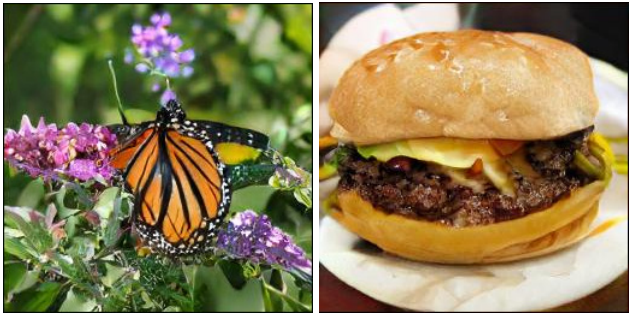
\includegraphics[width=\textwidth]{Slides/figures/GAN/BigGAN.PNG}
        \caption{Resultados de la arquitectura BigGAN\cite{brock2018large}.}
    \end{figure}
    
    \end{column}
    \hfill
    \begin{column}{.48\textwidth}
    
    \begin{figure}
        \centering
        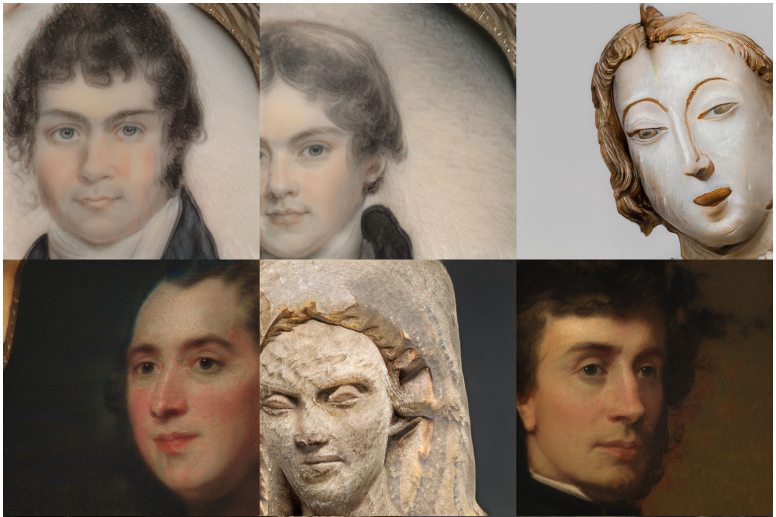
\includegraphics[width=\textwidth]{Slides/figures/GAN/Alias-FreeGAN.PNG}
        \caption{Resultados de la arquitectura Alias-Free GAN (StyleGAN-3)\cite{karras2021alias}.}
    \end{figure}

    \end{column}
    \end{columns}

\end{frame}

\begin{frame}{Domain-to-domain translation}

    El \alert{Domain-to-domain translation} es una aplicación \alert{no exclusiva} de las \gls{gan}. Sin embargo estas redes funcionan muy bien para esta aplicación.
    
    Es una de las aplicaciones \alert{más vistosas} y que más ha ayudado a la popularidad de las \gls{gan} en os últimos años.
    
    \begin{itemize}
        \item La idea es traducir un conjunto de datos de entrada de \alert{un dominio a otro distinto}.
    \end{itemize}

\end{frame}

\begin{frame}{Domain-to-domain translation: Ejemplos}

    \begin{columns}[T]
    \begin{column}{.48\textwidth}
    
    \begin{figure}
        \centering
        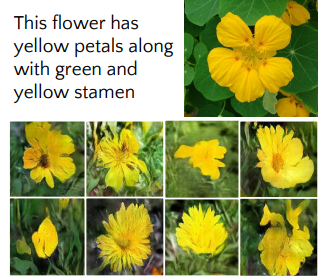
\includegraphics[width=\textwidth]{Slides/figures/GAN/TAC-GAN.PNG}
        \caption{Resultados de la arquitectura TAC-GAN\cite{dash2017tac}.}
    \end{figure}
    
    \end{column}
    \hfill
    \begin{column}{.55\textwidth}
    
    \begin{figure}
        \centering
        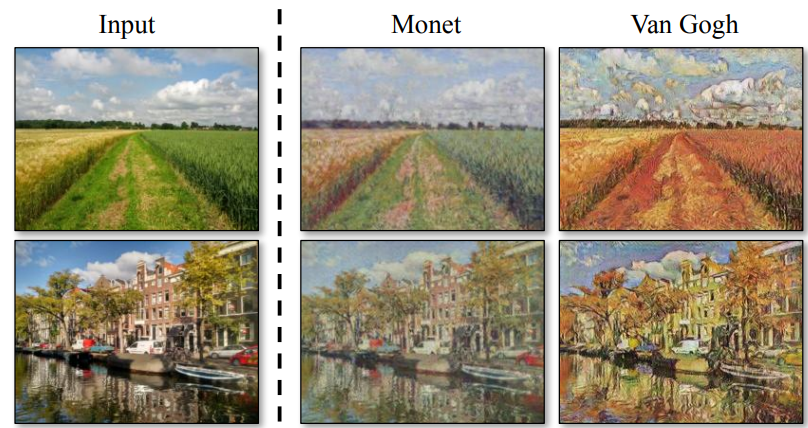
\includegraphics[width=\textwidth]{Slides/figures/GAN/CycleGAN.PNG}
        \caption{Resultados de la arquitectura CycleGAN\cite{zhu2017unpaired}.}
    \end{figure}

    \end{column}
    \end{columns}

\end{frame}

\begin{frame}{Data augmentation}

    Data Augmentation consiste en generar \alert{nuevos datos} de un dataset para aumentar el número de ejemplos. Esto es especialmente útil cuando se cuenta con conjuntos de datos \alert{insuficientes} para entrenar, por ejemplo, una red neuronal.
    
    También toma especial importancia cuando se cuenta con \alert{desbalanceo} entre clases de un dataset.
    
    Las \gls{gan} tienen como principal ventaja que generan nuevos datos muy similares a la distribución de datos original, pero sin copiar ni modificarlos directamente.
    
\end{frame}

\section{\gls{gan}: Arquitecturas}

\begin{frame}{\gls{acgan}\cite{odena2016conditional}}

    \begin{itemize}
        \item Capaz de separar en distintas \alert{clases} los datos con los que trata.
        \item Realiza un entrenamiento \alert{supervisado} usando las etiquetas del dataset.
        \item El discriminador distingue además de la \alert{veracidad} de cada dato, la clase a la que pertenece. De esta manera es capaz de aprender los distintos tipos de datos.
    \end{itemize}
    
    \begin{figure}
        \centering
        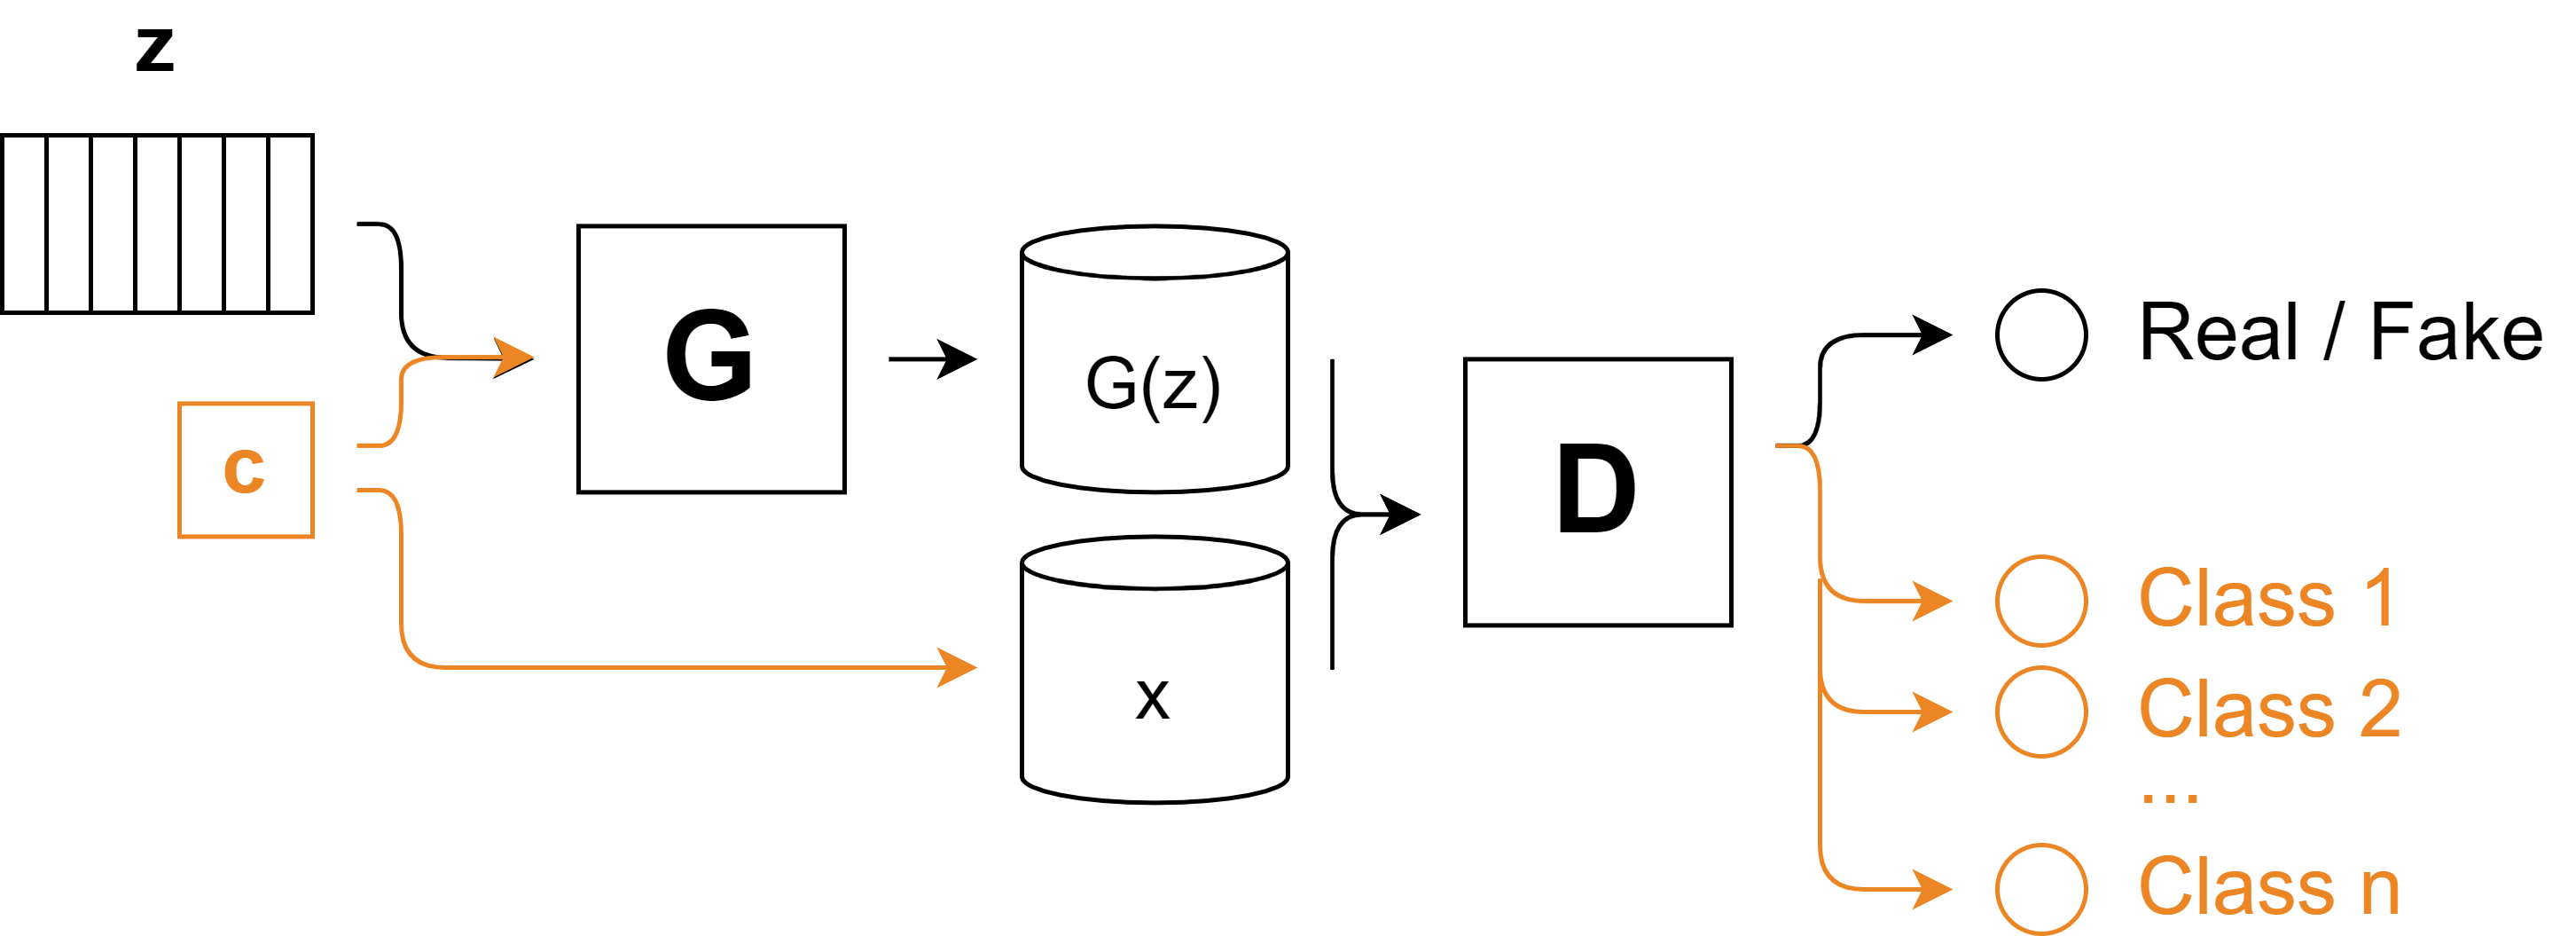
\includegraphics[width=\textwidth]{Slides/figures/GAN/ACGAN.png}
        \caption{Arquitectura de una ACGAN}
    \end{figure}
    
\end{frame}

\begin{frame}{\gls{acgan}\cite{odena2016conditional}}

    \begin{itemize}
        \item Capaz de separar en distintas \alert{clases} los datos con los que trata.
        \item Realiza un entrenamiento \alert{supervisado} usando las etiquetas del dataset.
        \item El discriminador distingue además de la \alert{veracidad} de cada dato, la clase a la que pertenece. De esta manera es capaz de aprender los distintos tipos de datos.
    \end{itemize}
    
    \begin{figure}
        \centering
        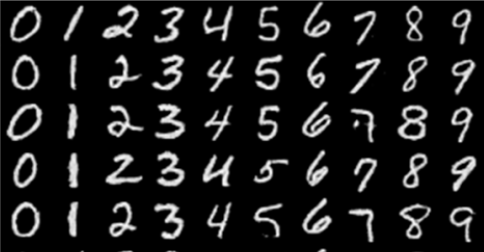
\includegraphics[width=0.6\textwidth]{Slides/figures/GAN/ACGAN Results.PNG}
        \caption{Resultados de una ACGAN para la generación de dígitos del dataset MNIST\cite{lecun1998mnist}}
    \end{figure}
    
\end{frame}

\begin{frame}{Image-to-Image Translation with Conditional Adversarial Nets (pix2pix)\cite{isola2017image}}

    \begin{itemize}
        \item La arquitectura \alert{pix2pix} fue presentada para realizar generación de imágenes \alert{condicionada} por una entrada, que \alert{también es una imagen}.
        \item La idea es traducir la imagen de entrada a otro \alert{dominio}, en lo que se conoce como \alert{image-to-image translation}.
    \end{itemize}
    
    \begin{figure}
        \centering
        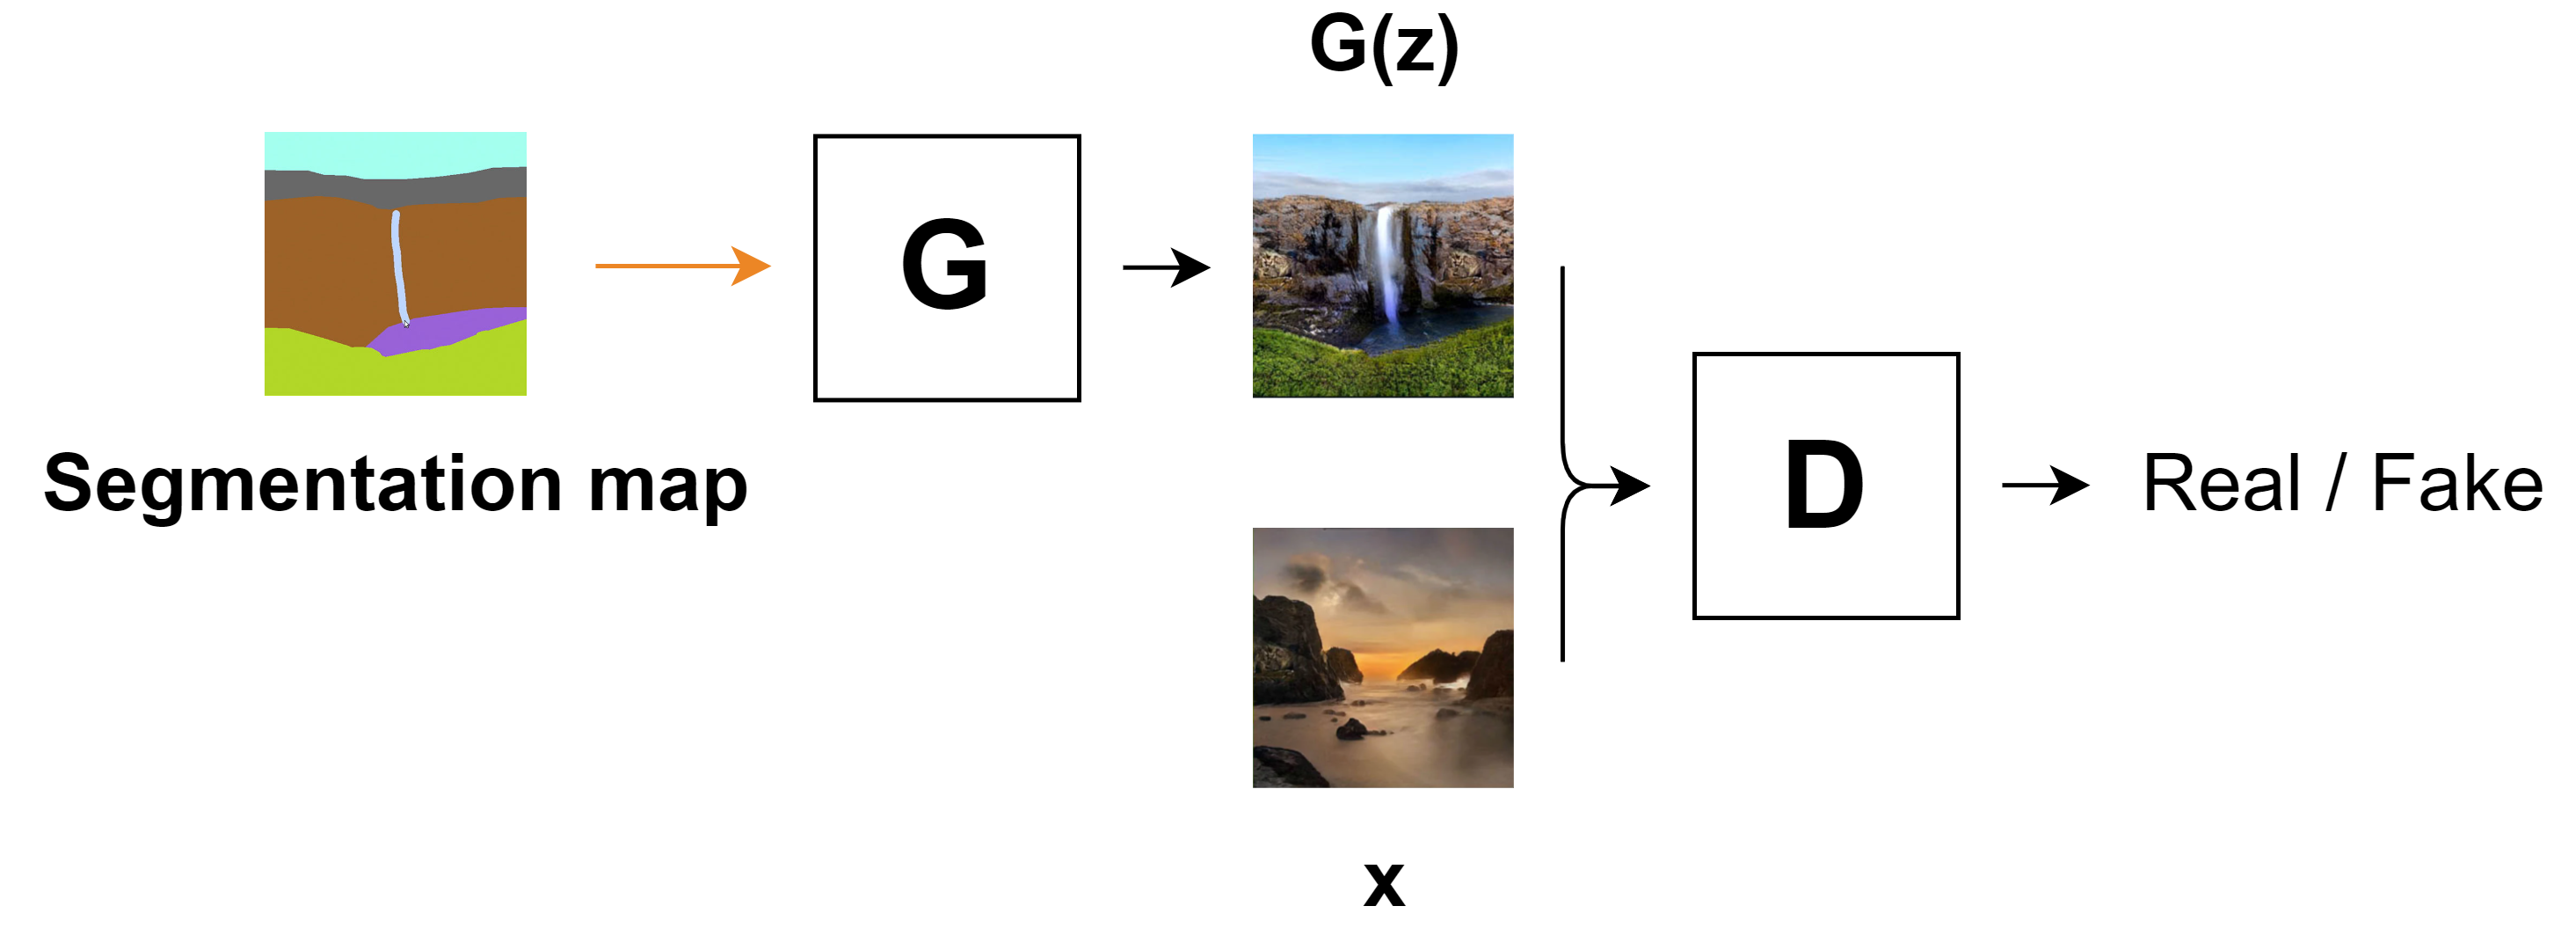
\includegraphics[width=0.85\textwidth]{Slides/figures/GAN/pix2pix.png}
        \caption{Arquitectura general de una pix2pix.}
    \end{figure}
    
\end{frame}

\begin{frame}{Image-to-Image Translation with Conditional Adversarial Nets (pix2pix)\cite{isola2017image}}

    \begin{itemize}
        \item El discriminador se encarga de juzgar la veracidad de cada uno de los \alert{parches} en los que se divide una imagen. Esta arquitectura se conoce como \alert{PatchGAN}\cite{isola2017image}.
        \item De esta manera se consigue que cada sección de la imagen sea realista.
    \end{itemize}
    
    \begin{figure}
        \centering
        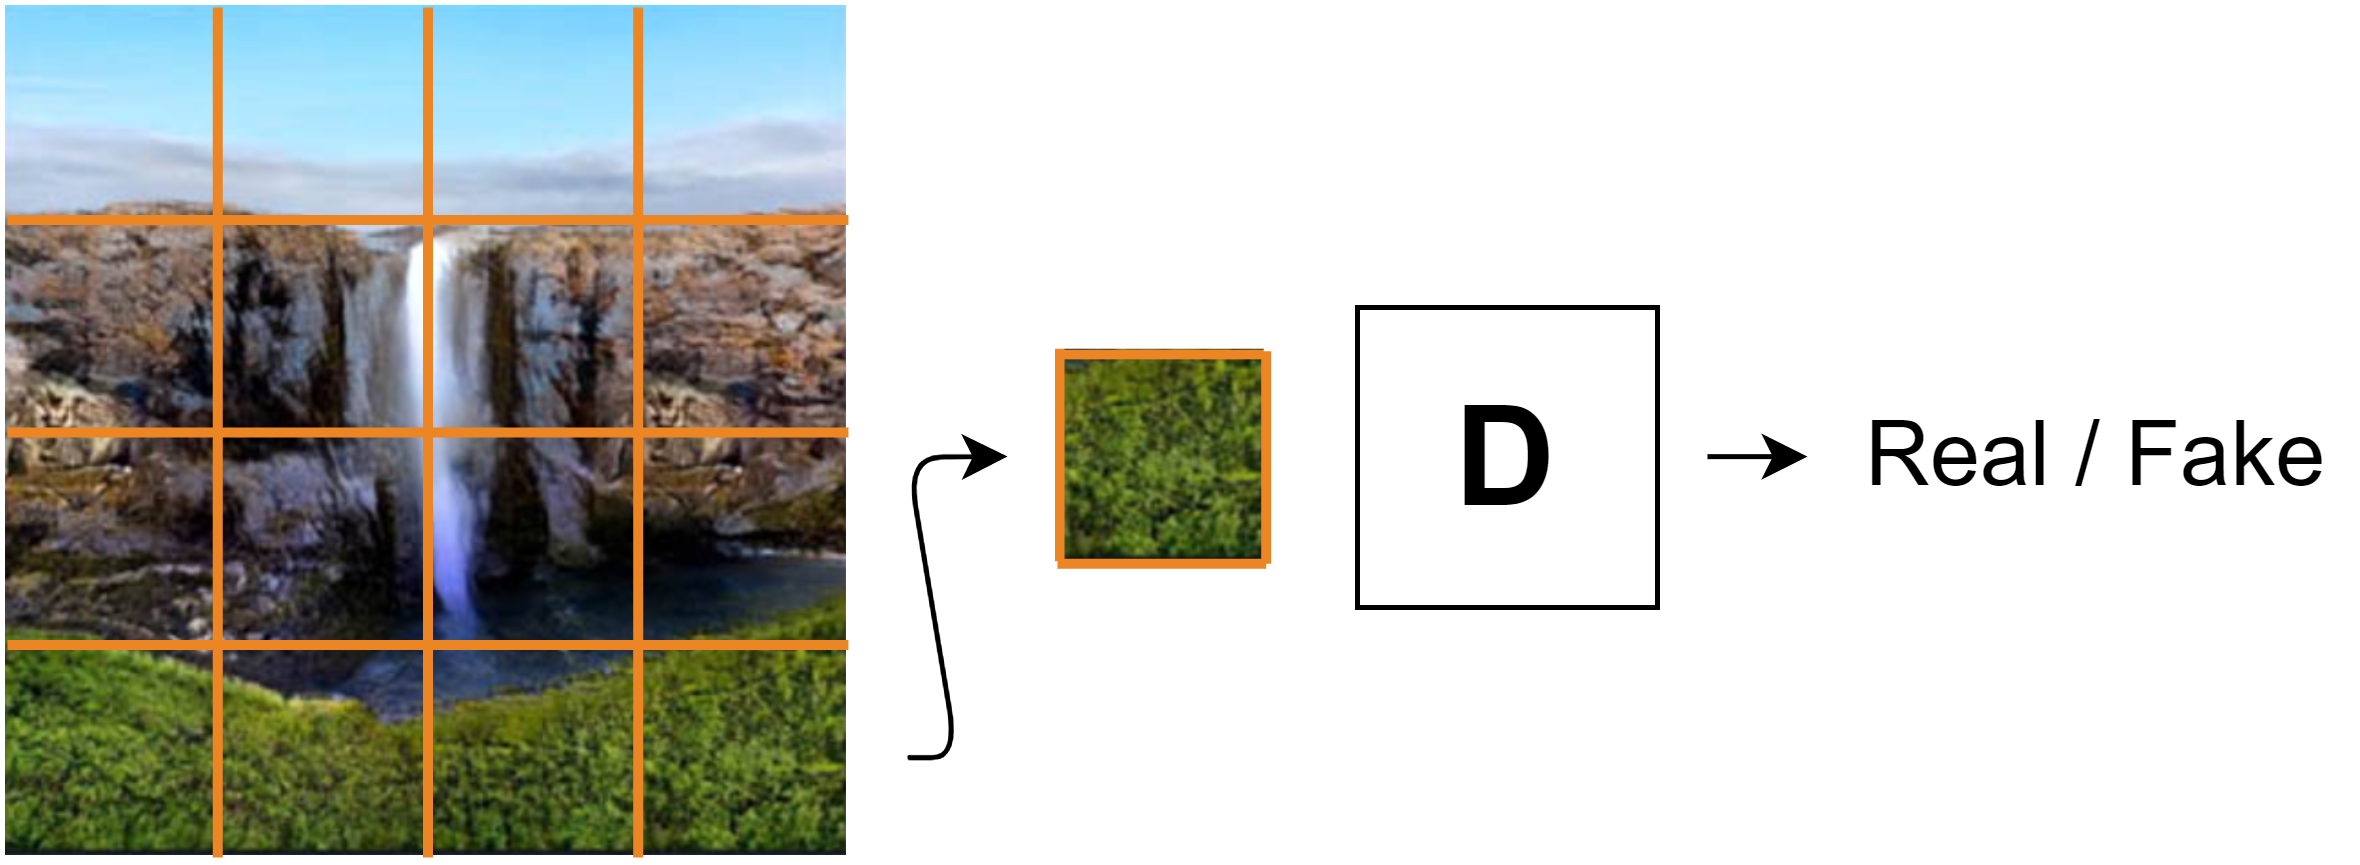
\includegraphics[width=0.9\textwidth]{Slides/figures/GAN/pix2pix Discriminador.png}
        \caption{Discriminador de la arquitectura PatchGAN\cite{isola2017image}.}
    \end{figure}
    
\end{frame}

\begin{frame}{Image-to-Image Translation with Conditional Adversarial Nets (pix2pix)\cite{isola2017image}}

    \begin{itemize}
        \item El nuevo discriminador necesita una \alert{función de pérdida} que permita unir la clasificación de todos los \alert{parches}.
    \end{itemize}
    
    \begin{equation}
        \large L=\sum\left[\log D\left(x_{i}\right)+\log \left(1-D\left(G\left(z_{i}\right)\right)\right)+\lambda L_{L 1}(G)\right]
    \end{equation}
    
    \begin{equation}
        \large L_{L 1}(G)=y-G(z, x)
    \end{equation}
    
\end{frame}

\begin{frame}{GauGAN\cite{park2019semantic}}

    \begin{itemize}
        \item Arquitectura presentada por \alert{NVIDIA} que consigue mejorar aún más los resultados de la \alert{pix2pix} y \alert{pix2pixHD}.
    \end{itemize}
    
    \begin{figure}
        \centering
        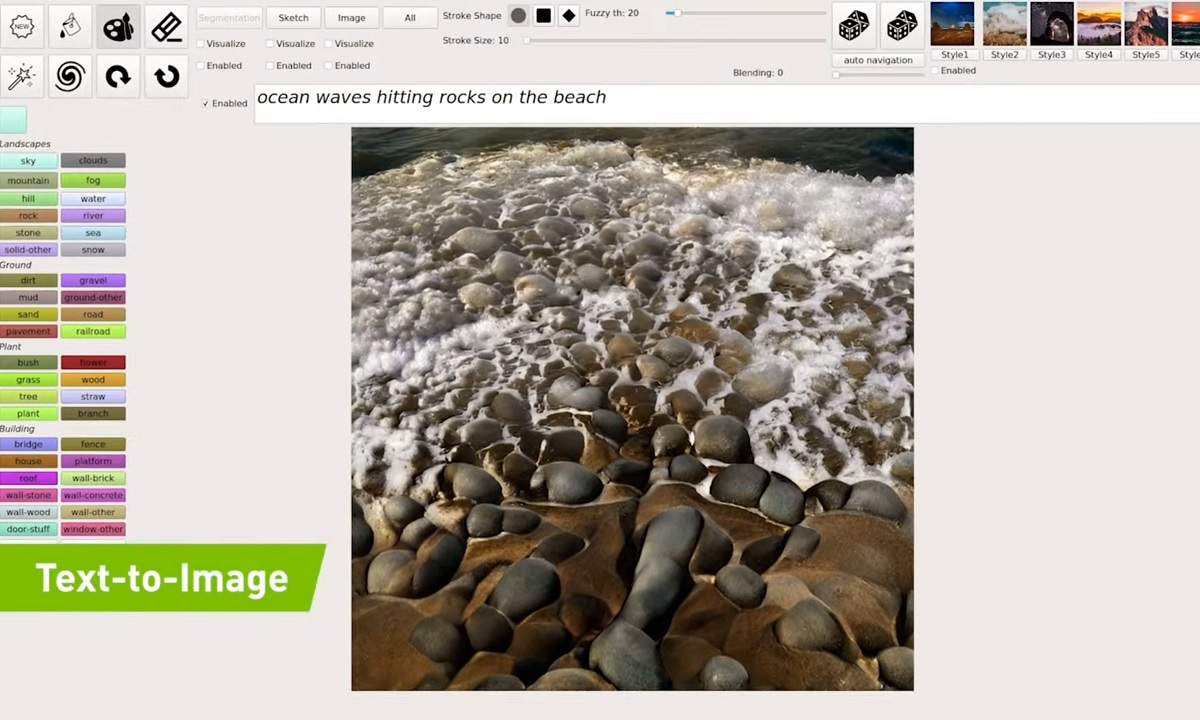
\includegraphics[width=0.75\textwidth]{Slides/figures/GAN/GauGAN2.jpg}
        \caption{\href{http://gaugan.org/gaugan2/}{http://gaugan.org/gaugan2/}.}
    \end{figure}
    
\end{frame}

\begin{frame}{Lineas de investigación de \gls{gan}}

    \begin{columns}[T]
    \begin{column}{0.48\textwidth}
    \alert{\Large Image-to-image translation}
    \begin{itemize}
        \item CGAN, 2014\cite{mirza2014conditional}
        \item \gls{acgan}, 2016\cite{odena2016conditional}
        \item pixpix, 2018\cite{isola2017image}
        \item CycleGAN, 2017\cite{isola2017image}
        \item DiscoGAN, 2017\cite{kim2017learning}
        \item GauGAN, 2019\cite{park2019semantic}
        \item CSGAN, 2019\cite{kancharagunta2019csgan}
    \end{itemize}
    \end{column}
    \hfill
    
    \begin{column}{.48\textwidth}
    \alert{\Large Mejoras en la calidad}
    \begin{itemize}
        \item DCGAN, 2016\cite{radford2015unsupervised}
        \item ProGAN, 2017\cite{karras2017progressive}
        \item StyleGAN, 2018\cite{karras2018style}
        \item Alias-FreeGAN, 2021\cite{karras2021alias}
        \item CSGAN, 2021\cite{kancharagunta2019csgan}
    \end{itemize}
    \end{column}
    \end{columns}
    
\end{frame}

\begin{frame}{Lineas de investigación de \gls{gan}}

    \begin{columns}[T]
    \begin{column}{0.48\textwidth}
    \alert{\Large Super resolution}
    \begin{itemize}
        \item SRGAN, 2017\cite{ledig2017photo}
        \item srcaGAN, 2021\cite{liu2021super}
        \item WSRGAN, 2021\cite{cao2021weighted}
    \end{itemize}
    \end{column}
    \hfill
    
    \begin{column}{.48\textwidth}
    \alert{\Large Crecimiento de las redes}
    \begin{itemize}
        \item ProGAN, 2017\cite{karras2017progressive}
        \item DGGAN, 2021\cite{liu2021dynamically}
    \end{itemize}
    \end{column}
    \end{columns}
    
\end{frame}

\addcontentsline{toc}{section}{Referencias}

\begin{frame}[allowframebreaks]{Referencias}
    \bibliographystyle{abbrv}
    \bibliography{references.bib}
\end{frame}

\begin{frame}{Contribuciones de las diapositivas}
\begin{itemize}
    \item \textbf{Autor original de las diapositivas:} Guillermo Iglesias Hernández
\end{itemize}
\end{frame}

\end{document}